\documentclass[11pt,a4paper]{report}
\usepackage[utf8]{inputenc}
\usepackage[portuguese]{babel}
\usepackage[T1]{fontenc}
\usepackage{amsmath}
\usepackage{amsfonts}
\usepackage{amssymb}
\usepackage{graphicx}
\title{Relatório sobre o ajuste dos offsets dos satélites irregulares}
\author{Altair Ramos}
\begin{document}

\chapter*{Ajuste}

\begin{equation}
p[0]\sin\left(\frac{2\pi}{p[1]*365.25}\times (t - 2451544.5) + p[2]\right) + p[3]\sin(f) + p[4]\cos(f) + p[5]
\end{equation}


\chapter*{Ananke}
\section*{Ascensão Reta}

\begin{figure}[h]
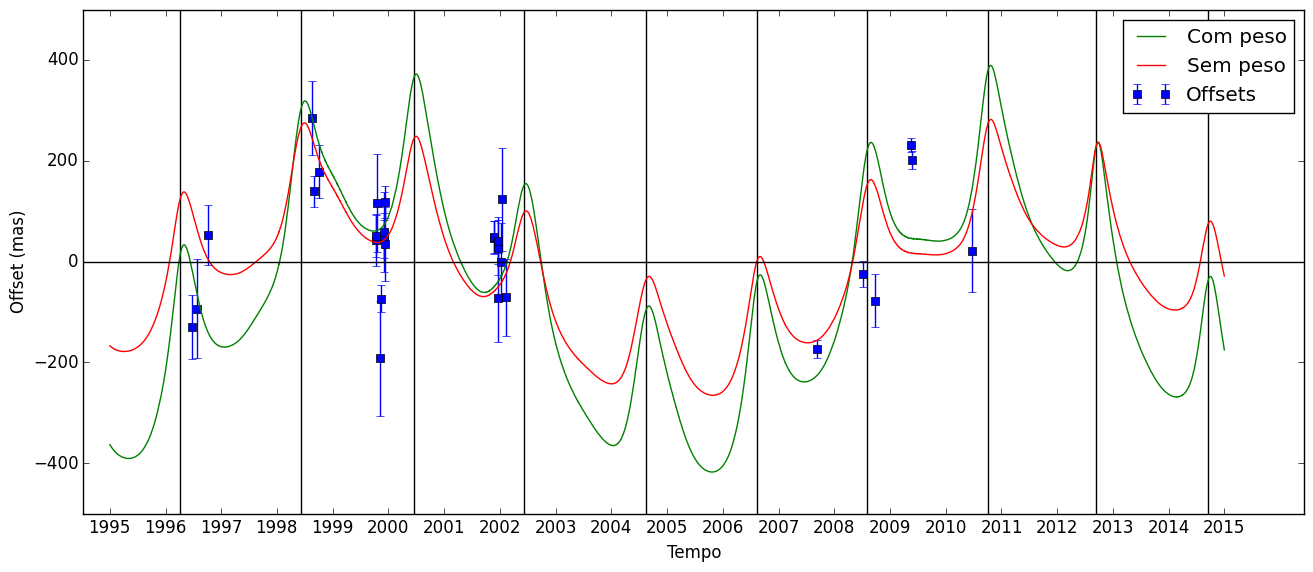
\includegraphics[scale=0.35]{Ananke/RA.png} 
\end{figure}

\begin{figure}[h]
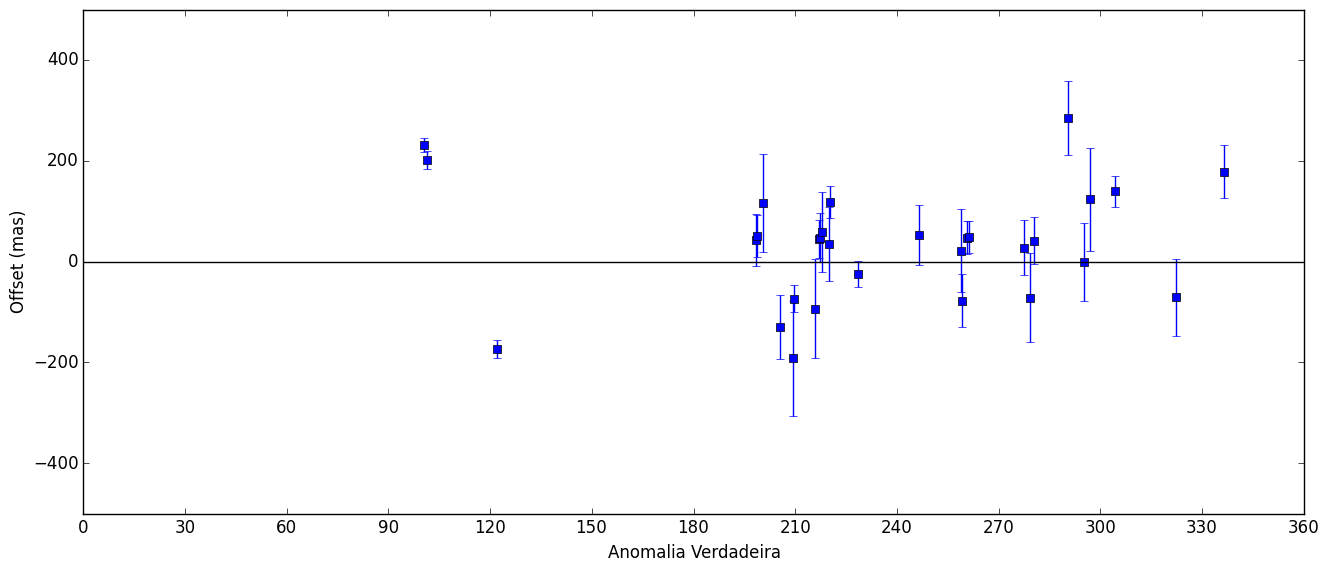
\includegraphics[scale=0.35]{Ananke/RA_anom.png}  
\end{figure}

\begin{table}[h!]
\caption{\label{Tab: Ananke-RA} Resultados dos ajustes para Ananke - RA}
\begin{centering}
\begin{tabular}{cccc}
\hline
\hline
Parâmetro & Com peso & Sem peso & Unidade\tabularnewline
\hline
p[0] & 246 $\pm$ 39 & 160 $\pm$ 43 & mas\\
p[1] & 10.8 $\pm$ 0.5 & 12.0 $\pm$ 0.9 & anos\\
p[2] & 0.09 $\pm$ 0.15 & 0.4 $\pm$ 0.1 & rad\\
p[3] & 60 $\pm$ 29 & 44 $\pm$ 39 & mas\\
p[4] & 152 $\pm$ 37 & 111 $\pm$ 32 & mas\\
p[5] & -20 $\pm$ 37 & 5 $\pm$ 37 & mas\\
Residuo & 571 & 451 & mas\\
\hline 
\end{tabular} 
\par\end{centering}
\end{table}

\section*{Declinação}


\begin{figure}[h]
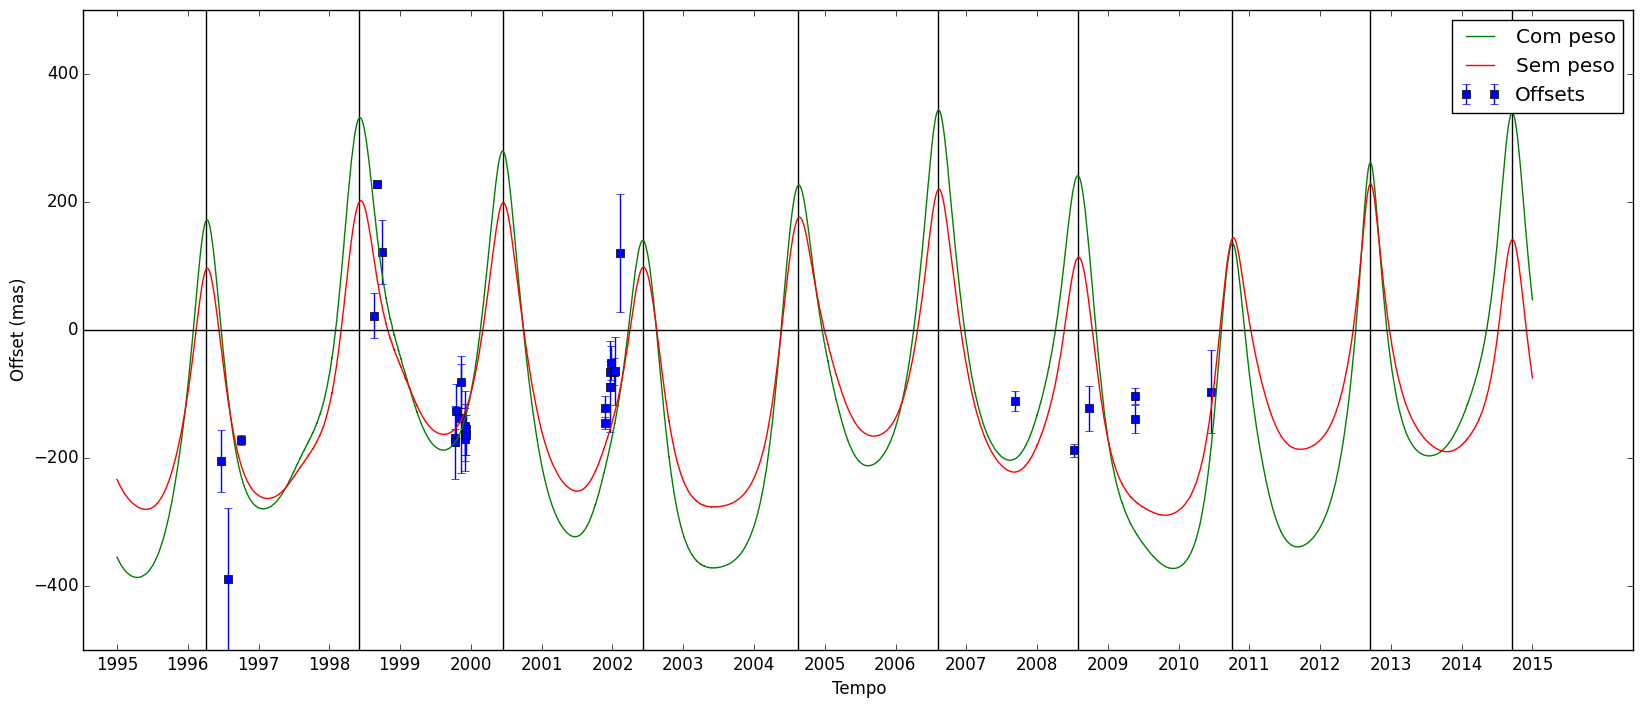
\includegraphics[scale=0.35]{Ananke/DEC.png} 
\end{figure}

\begin{figure}[h]
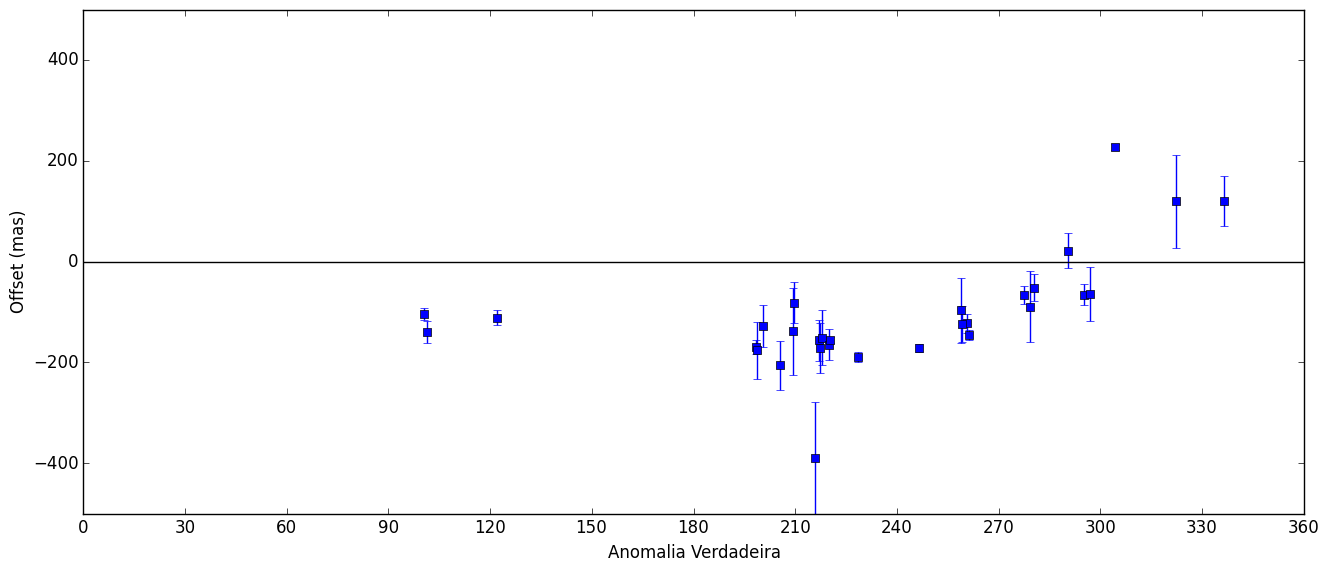
\includegraphics[scale=0.35]{Ananke/DEC_anom.png}  
\end{figure}

\begin{table}[h!]
\caption{\label{Tab: Ananke-DEC} Resultados dos ajustes para Ananke - DEC}
\begin{centering}
\begin{tabular}{cccc}
\hline
\hline
Parâmetro & Com peso & Sem peso & Unidade\tabularnewline
\hline
p[0] & 105 $\pm$ 8 & 66 $\pm$ 12 & mas\\
p[1] & 7.6 $\pm$ 0.2 & 6.6 $\pm$ 0.4 & anos\\
p[2] & 0.80 $\pm$ 0.08 & 0.5 $\pm$ 0.3 & rad\\
p[3] & 9 $\pm$ 11 & 18 $\pm$ 18 & mas\\
p[4] & 260 $\pm$ 10 & 194 $\pm$ 19 & mas\\
p[5] & -22 $\pm$ 13 & -34 $\pm$ 16 & mas\\
Residuo & 338 & 253 & mas\\
\hline 
\end{tabular} 
\par\end{centering}
\end{table}

\chapter*{Carme}
\section*{Ascensão Reta}

\begin{figure}[h]
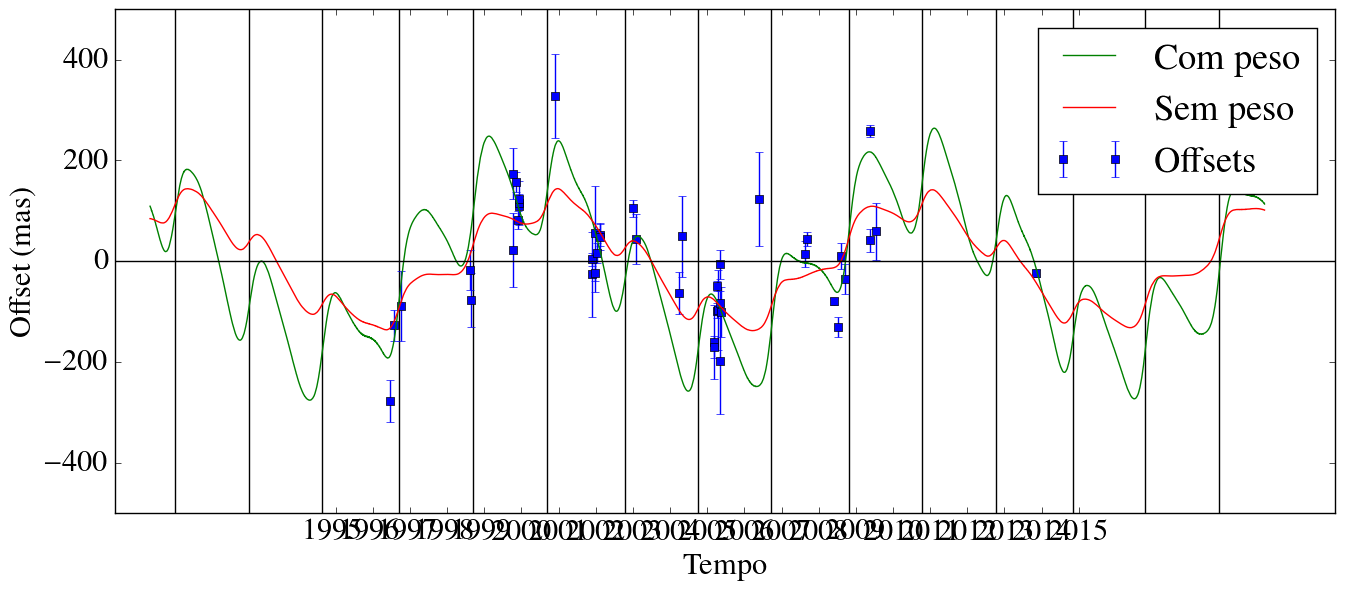
\includegraphics[scale=0.35]{Carme/RA.png} 
\end{figure}

\begin{figure}[h]
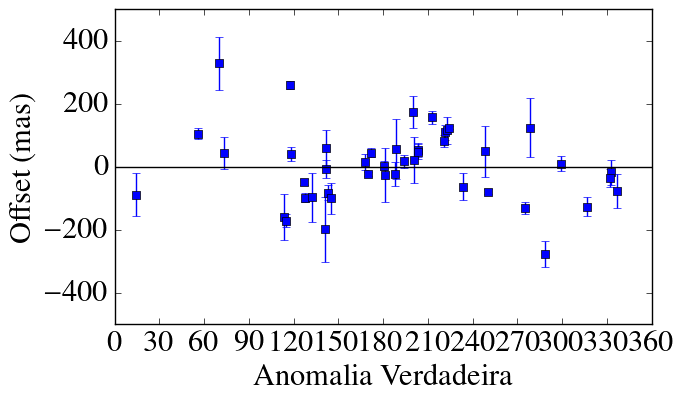
\includegraphics[scale=0.35]{Carme/RA_anom.png}  
\end{figure}

\begin{table}[h!]
\caption{\label{Tab: Carme-RA} Resultados dos ajustes para Carme - RA}
\begin{centering}
\begin{tabular}{cccc}
\hline
\hline
Parâmetro & Com peso & Sem peso & Unidade\tabularnewline
\hline
p[0] & 167 $\pm$ 14 & 112 $\pm$ 20 & mas\\
p[1] & 10.7 $\pm$ 0.2 & 9.9 $\pm$ 0.7 & anos\\
p[2] & 0.0 $\pm$ 0.1 & -0.4 $\pm$ 0.3 & rad\\
p[3] & 104 $\pm$ 16 & 33 $\pm$ 22 & mas\\
p[4] & -17 $\pm$ 20 & 0 $\pm$ 24 & mas\\
p[5] & -4 $\pm$ 15 & 0 $\pm$ 17 & mas\\
Residuo & 662 & 556 & mas\\
\hline 
\end{tabular} 
\par\end{centering}
\end{table}

\section*{Declinação}

\begin{figure}[h]
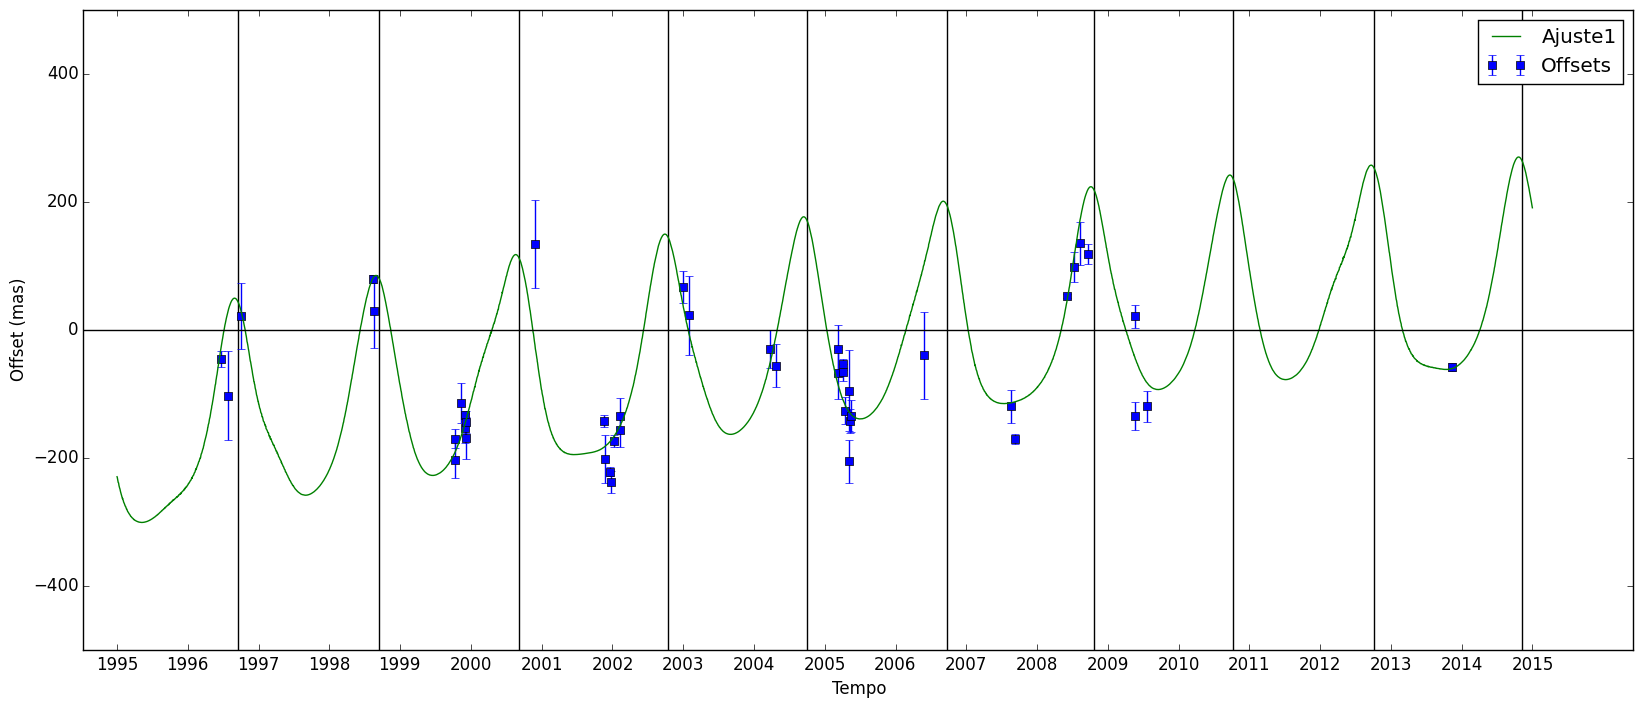
\includegraphics[scale=0.35]{Carme/DEC.png} 
\end{figure}

\begin{figure}[h]
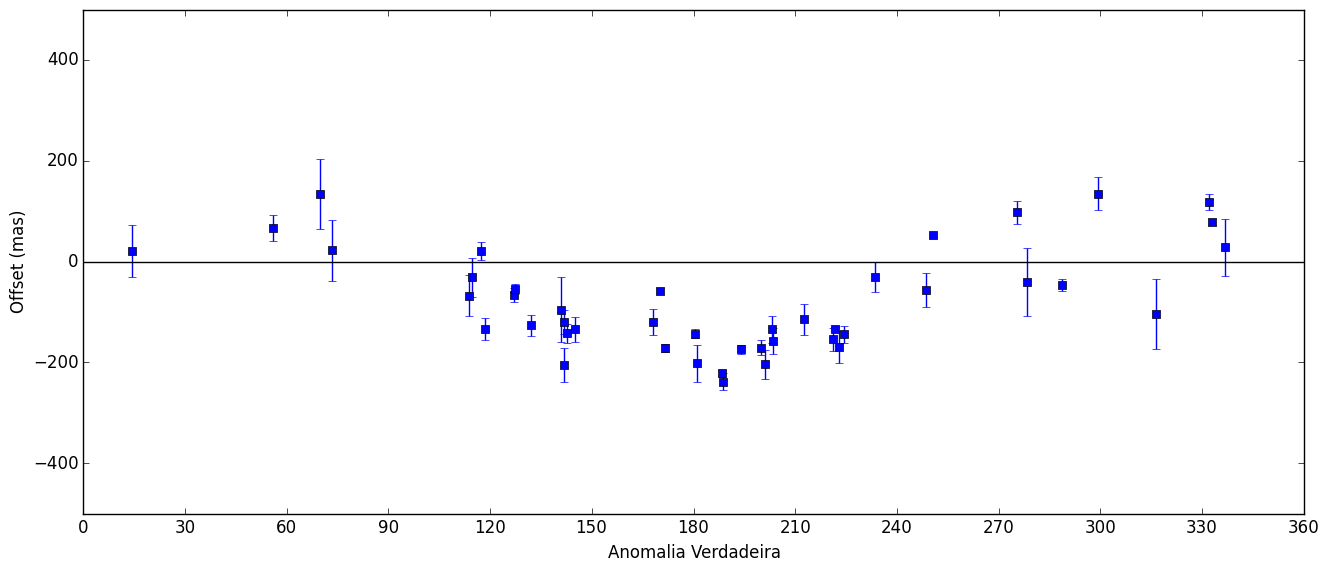
\includegraphics[scale=0.35]{Carme/DEC_anom.png}  
\end{figure}

\begin{table}[h!]
\caption{\label{Tab: Carme-DEC} Resultados dos ajustes para Carme - DEC}
\begin{centering}
\begin{tabular}{cccc}
\hline
\hline
Parâmetro & Com peso & Sem peso & Unidade\tabularnewline
\hline
p[0] & 0.036 $\pm$ 0.003 & 0.034 $\pm$ 0.005 & mas\\
p[1] & 70 $\pm$ 30 & 71 $\pm$ 22 & anos\\
p[2] & -8 $\pm$ 18 & 9 $\pm$ 11 & rad\\
p[3] & 182 $\pm$ 15 & 153 $\pm$ 11 & mas\\
p[4] & -39 $\pm$ 11 & -58 $\pm$ 10 & mas\\
Residuo & 325 & 281 & mas\\
\hline 
\end{tabular} 
\par\end{centering}
\end{table}

\chapter*{Elara}
\section*{Ascensão Reta}

\begin{figure}[h]
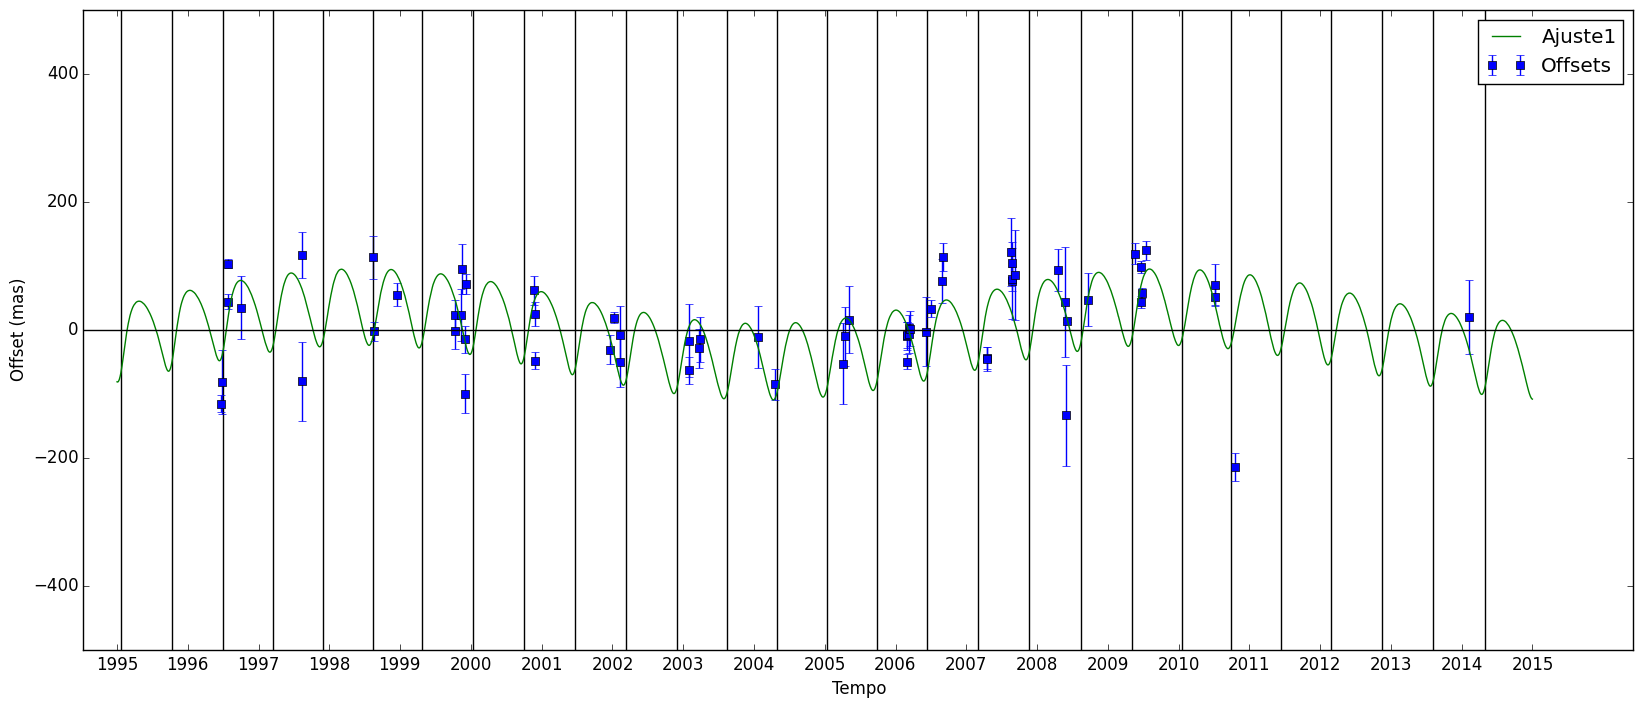
\includegraphics[scale=0.35]{Elara/RA.png} 
\end{figure}

\begin{figure}[h]
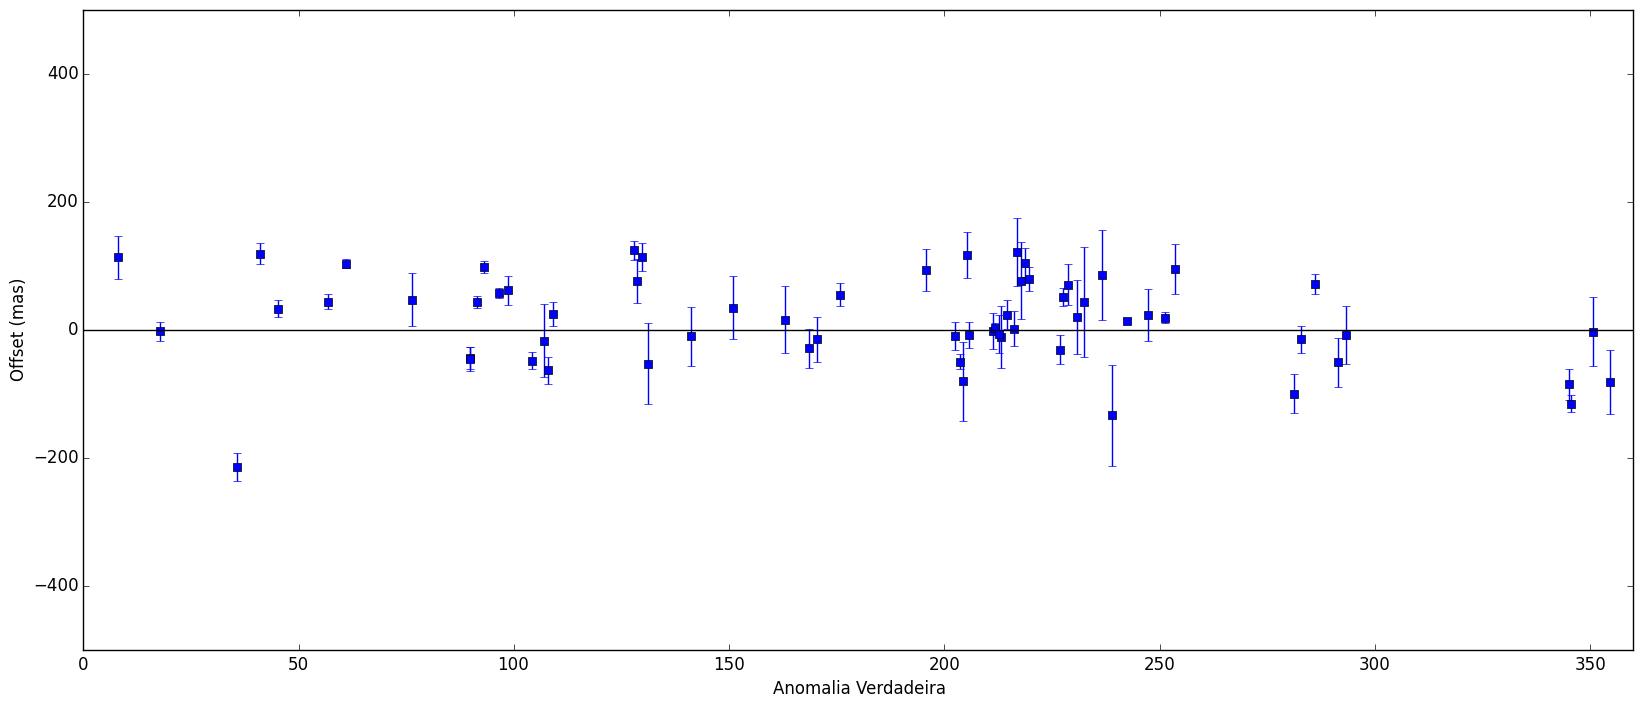
\includegraphics[scale=0.35]{Elara/RA_anom.png}  
\end{figure}

\begin{table}[h!]
\caption{\label{Tab: Elara-RA} Resultados dos ajustes para Elara - RA}
\begin{centering}
\begin{tabular}{cccc}
\hline
\hline
Parâmetro & Com peso & Sem peso & Unidade\tabularnewline
\hline
p[0] & -42 $\pm$ 17 & -63 $\pm$ 20 & mas\\
p[1] & 11 $\pm$ 2 & 8.5 $\pm$ 0.8 & anos\\
p[2] & -0.7 $\pm$ 0.4 & -1.4 $\pm$ 0.4 & rad\\
p[3] & 33 $\pm$ 13 & 27 $\pm$ 18 & mas\\
p[4] & -49 $\pm$ 23 & -57 $\pm$ 21 & mas\\
p[5] & -7 $\pm$ 14 & -23 $\pm$ 15 & mas\\
Residuo & 848 & 792 & mas\\
\hline 
\end{tabular} 
\par\end{centering}
\end{table}

\section*{Declinação}

\begin{figure}[h]
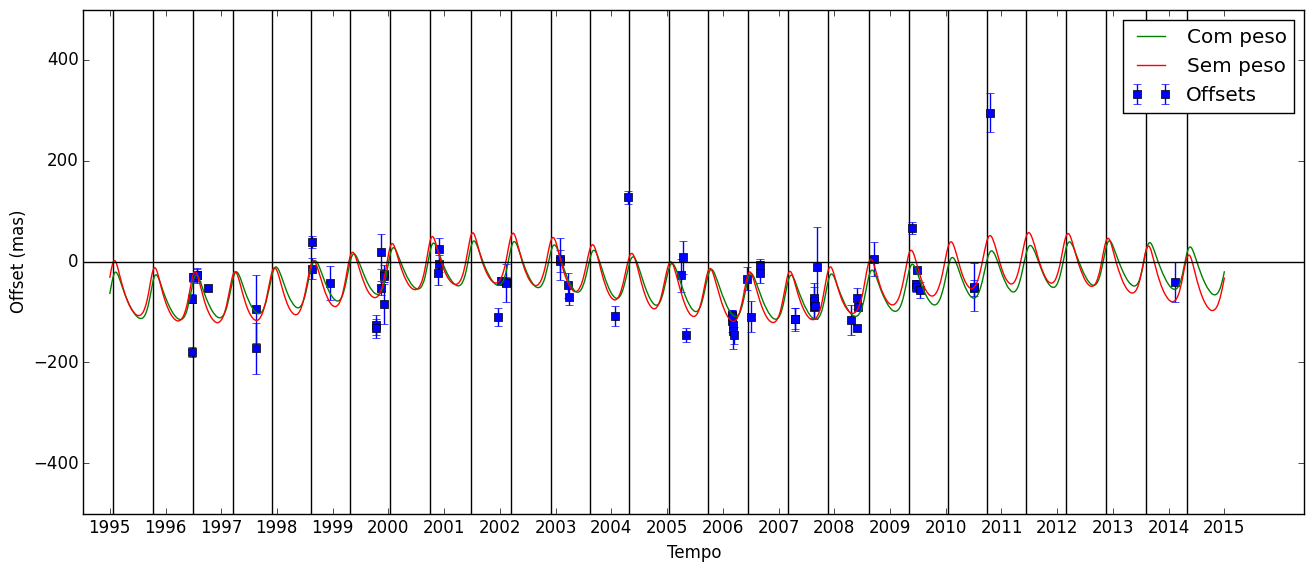
\includegraphics[scale=0.35]{Elara/DEC.png} 
\end{figure}

\begin{figure}[h]
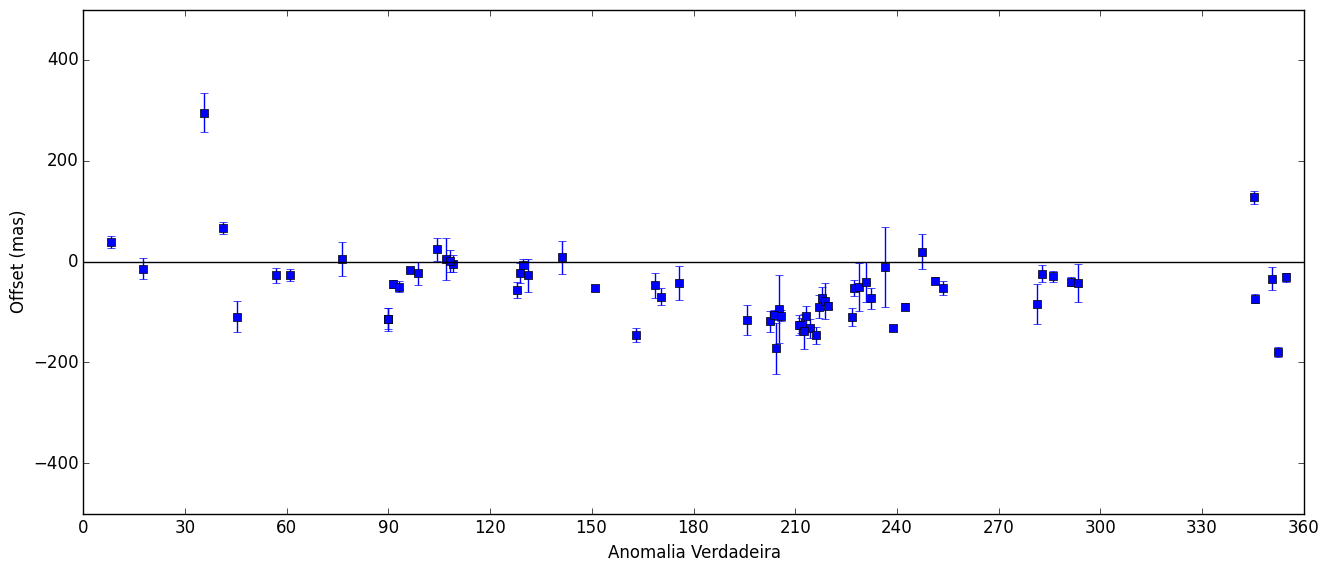
\includegraphics[scale=0.35]{Elara/DEC_anom.png}  
\end{figure}

\begin{table}[h!]
\caption{\label{Tab: Elara-DEC} Resultados dos ajustes para Elara - DEC}
\begin{centering}
\begin{tabular}{cccc}
\hline
\hline
Parâmetro & Com peso & Sem peso & Unidade\tabularnewline
\hline
p[0] & 34 $\pm$ 8 & 39 $\pm$ 10 & mas\\
p[1] & 11.1 $\pm$ 1.2 & 9.8 $\pm$ 0.9 & anos\\
p[2] & 0.6 $\pm$ 0.4 & 0.4 $\pm$ 0.4 & rad\\
p[3] & 32 $\pm$ 8 & 26 $\pm$ 10 & mas\\
p[4] & 29 $\pm$ 8 & 42 $\pm$ 11 & mas\\
p[5] & -37 $\pm$ 7 & -31 $\pm$ 8 & mas\\
Residuo & 461 & 445 & mas\\
\hline 
\end{tabular} 
\par\end{centering}
\end{table}

\chapter*{Himalia}
\section*{Ascensão Reta}

\begin{figure}[h]
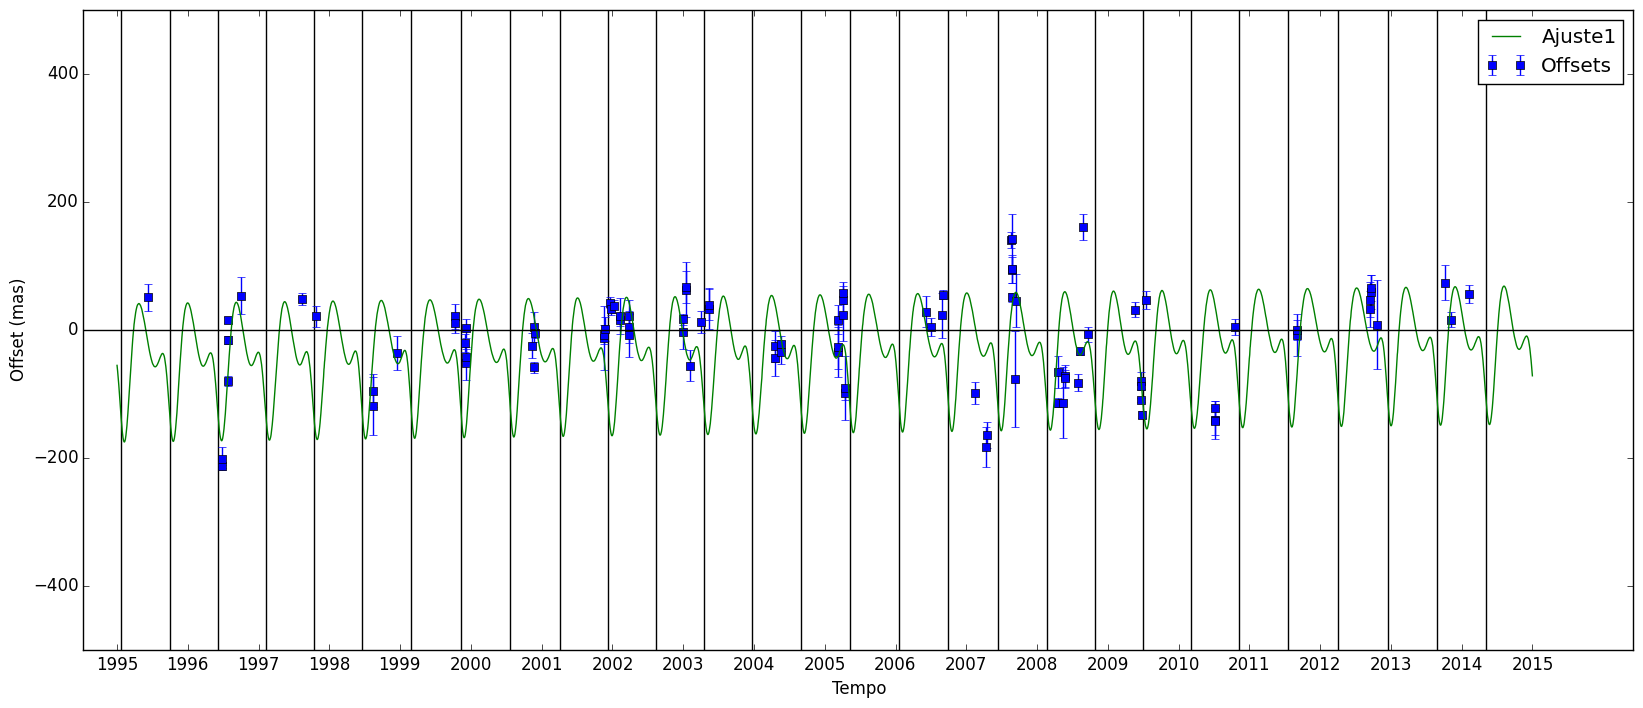
\includegraphics[scale=0.35]{Himalia/RA.png} 
\end{figure}

\begin{figure}[h]
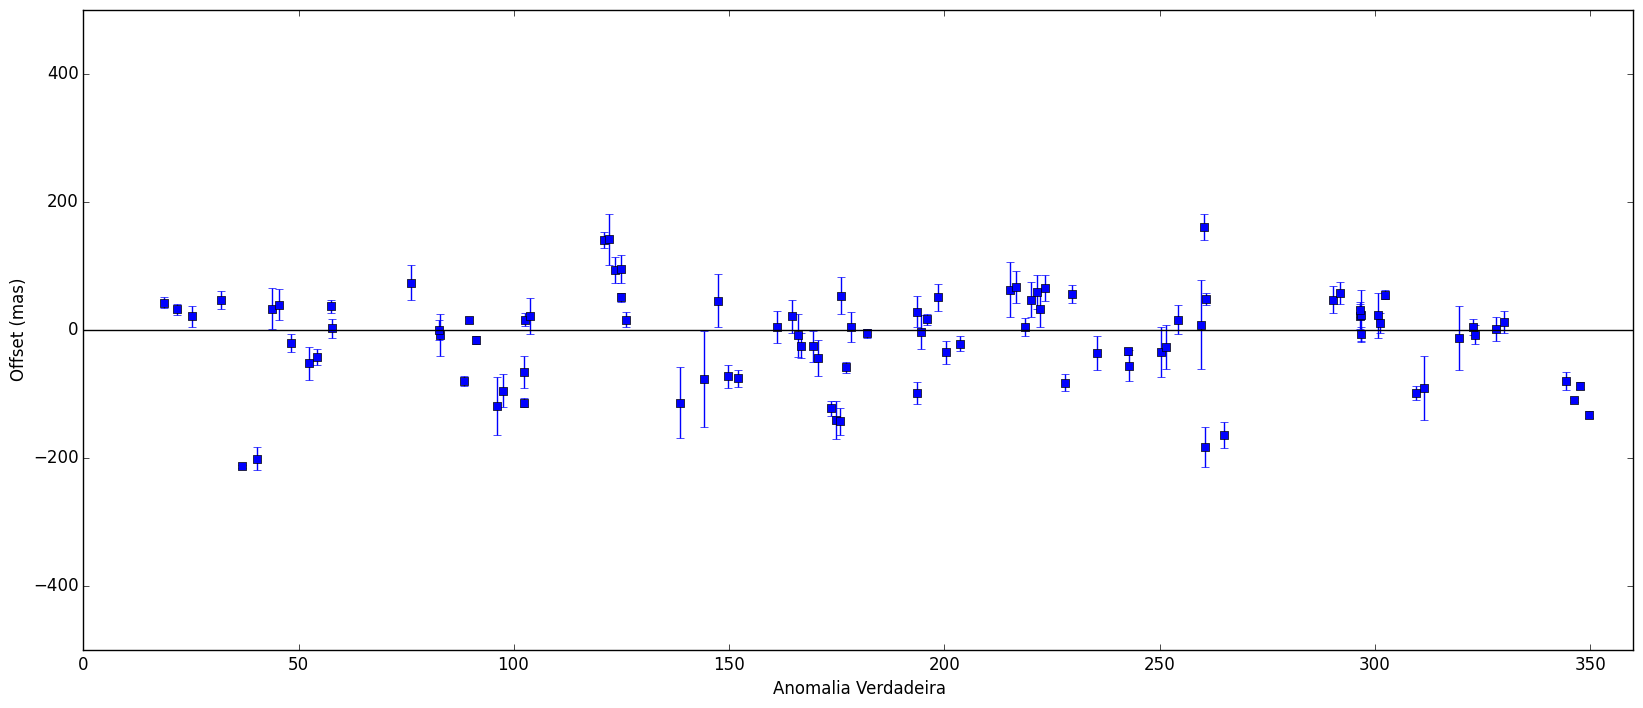
\includegraphics[scale=0.35]{Himalia/RA_anom.png}  
\end{figure}

\begin{table}[h!]
\caption{\label{Tab: Himalia-RA} Resultados dos ajustes para Himalia - RA}
\begin{centering}
\begin{tabular}{cccc}
\hline
\hline
Parâmetro & Com peso & Sem peso & Unidade\tabularnewline
\hline
p[0] & 71 $\pm$ 24 & 49 $\pm$ 19 & mas\\
p[1] & 18 $\pm$ 8 & 12 $\pm$ 2 & anos\\
p[2] & 0.1 $\pm$ 0.8 & 0.2 $\pm$ 0.7 & rad\\
p[3] & 0 $\pm$ 21 & -17 $\pm$ 21 & mas\\
p[4] & -55 $\pm$ 17 & -36 $\pm$ 21 & mas\\
p[5] & -49 $\pm$ 36 & -32 $\pm$ 14 & mas\\
Residuo & 1388 & 1348 & mas\\
\hline 
\end{tabular} 
\par\end{centering}
\end{table}

\section*{Declinação}

\begin{figure}[h]
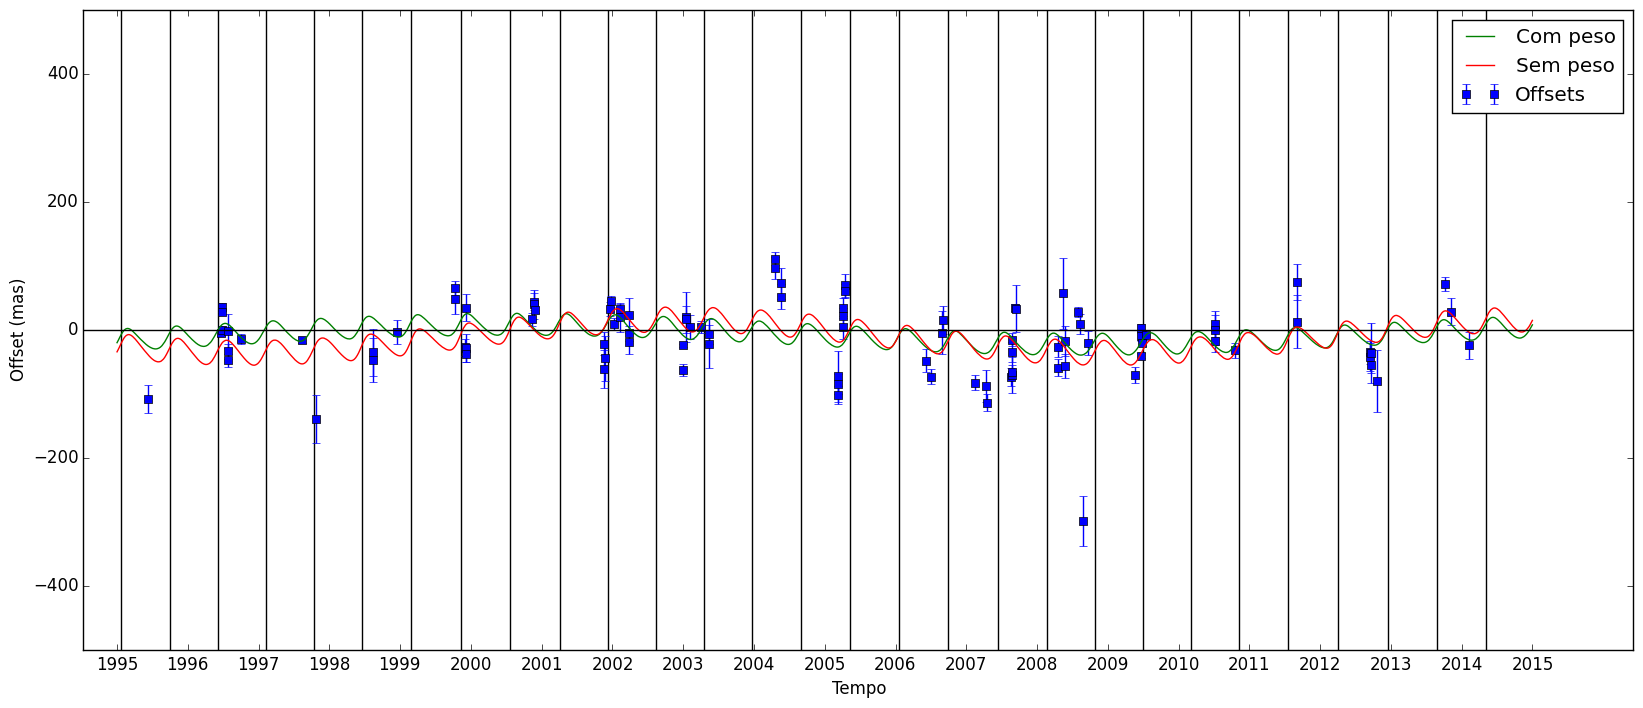
\includegraphics[scale=0.35]{Himalia/DEC.png} 
\end{figure}

\begin{figure}[h]
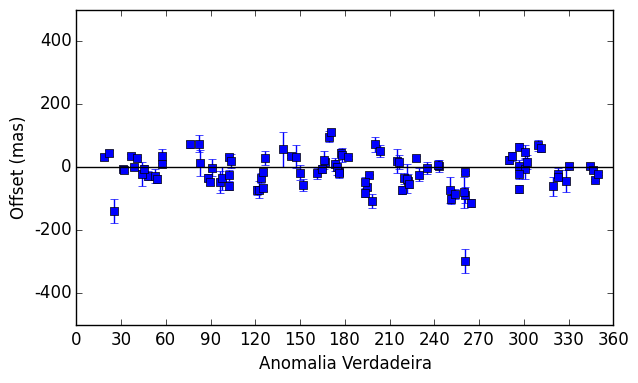
\includegraphics[scale=0.35]{Himalia/DEC_anom.png}  
\end{figure}

\begin{table}[h!]
\caption{\label{Tab: Himalia-DEC} Resultados dos ajustes para Himalia - DEC}
\begin{centering}
\begin{tabular}{cccc}
\hline
\hline
Parâmetro & Com peso & Sem peso & Unidade\tabularnewline
\hline
p[0] & 15 $\pm$ 5 & 2 $\pm$ 7 & mas\\
p[1] & 16 $\pm$ 3 & 12.2 $\pm$ 1.6 & anos\\
p[2] & 1.3 $\pm$ 0.43 & 0.0 $\pm$ 0.5 & rad\\
p[3] & 15 $\pm$ 6 & 19 $\pm$ 8 & mas\\
p[4] & 7 $\pm$ 5 & 7 $\pm$ 5 & mas\\
p[5] & -7 $\pm$ 4 & -7 $\pm$ 4 & mas\\
Residuo & 533 & 513 & mas\\
\hline 
\end{tabular} 
\par\end{centering}
\end{table}

\chapter*{Lysithea}
\section*{Ascensão Reta}

\begin{figure}[h]
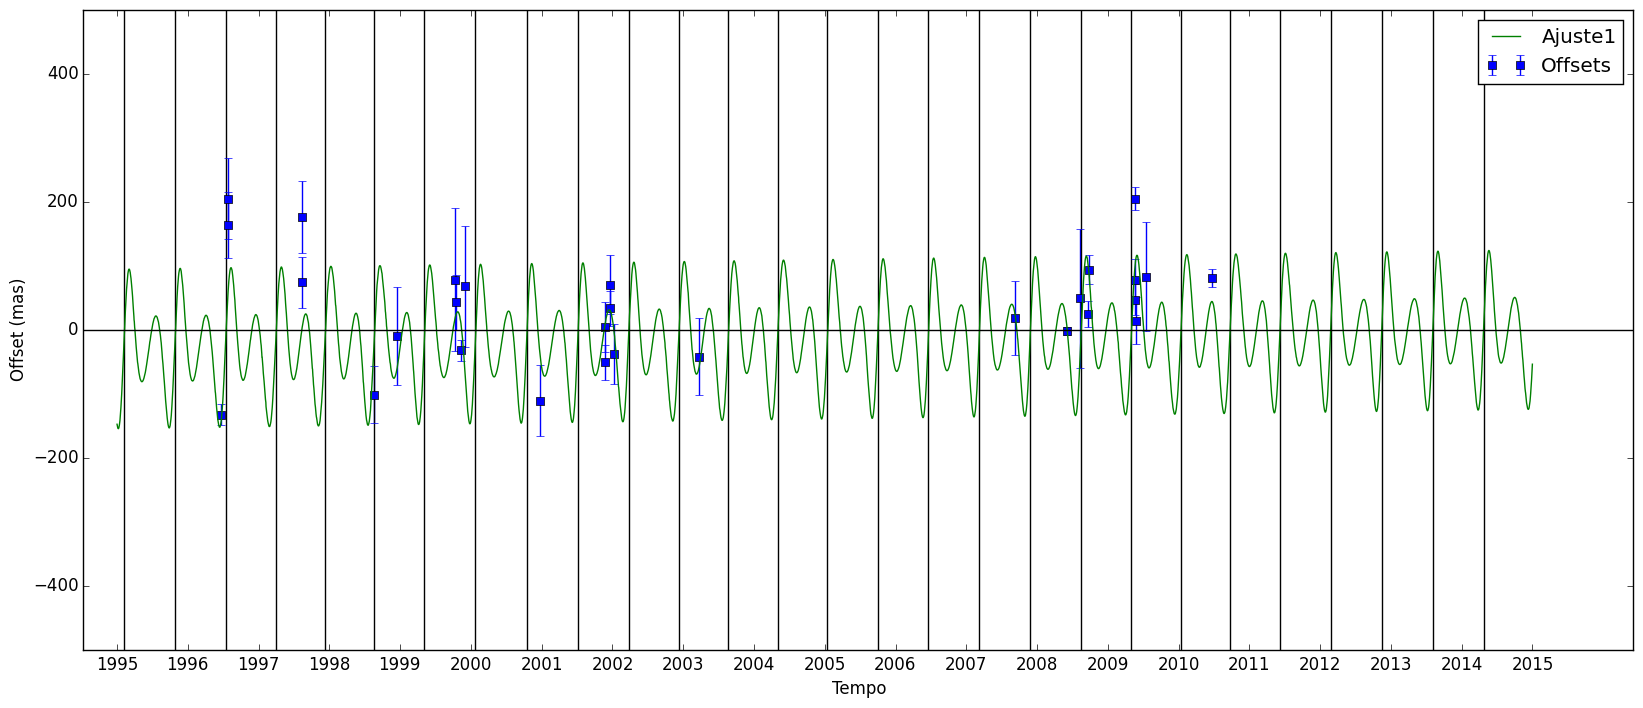
\includegraphics[scale=0.35]{Lysithea/RA.png} 
\end{figure}

\begin{figure}[h]
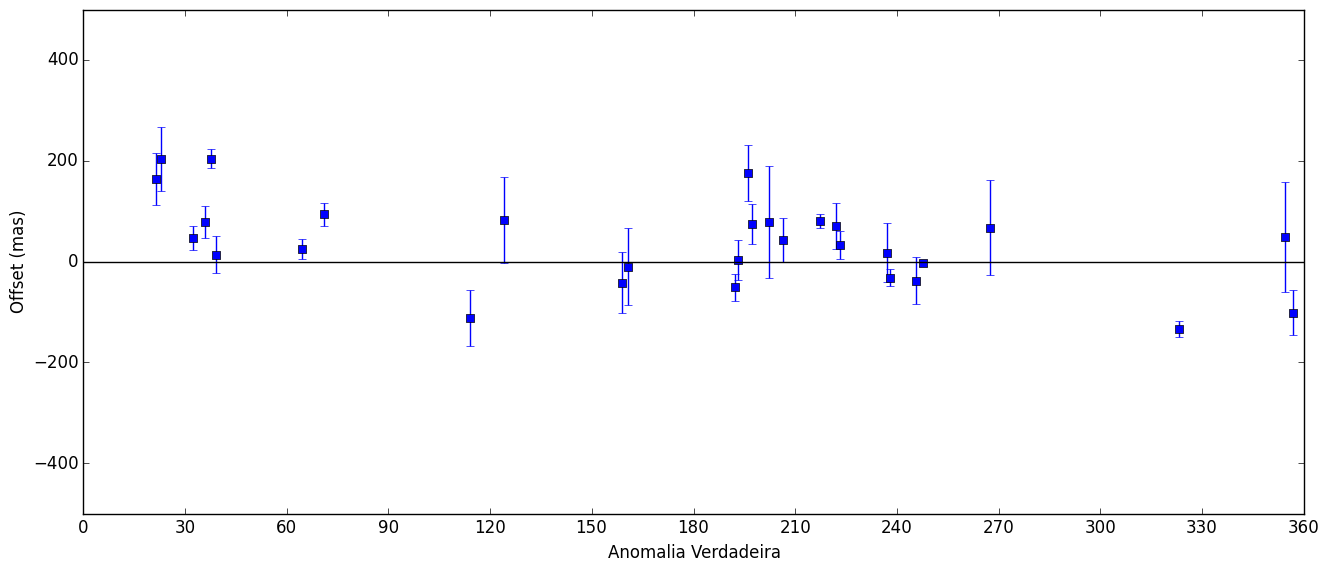
\includegraphics[scale=0.35]{Lysithea/RA_anom.png}  
\end{figure}

\begin{table}[h!]
\caption{\label{Tab: Lysithea-RA} Resultados dos ajustes para Lysithea - RA}
\begin{centering}
\begin{tabular}{cccc}
\hline
\hline
Parâmetro & Com peso & Sem peso & Unidade\tabularnewline
\hline
p[0] & 88 $\pm$ 37 & 117 $\pm$ 350 & mas\\
p[1] & 10.8 $\pm$ 0.9 & 24 $\pm$ 49 & anos\\
p[2] & 0.5 $\pm$ 0.4 & 2.3 $\pm$ 1.6 & rad\\
p[3] & 67 $\pm$ 27 & 12 $\pm$ 28 & mas\\
p[4] & -38 $\pm$ 33 & -24 $\pm$ 26 & mas\\
p[5] & -16 $\pm$ 28 & 79 $\pm$ 370 & mas\\
Residuo & 494 & 397 & mas\\
\hline 
\end{tabular} 
\par\end{centering}
\end{table}

\section*{Declinação}

\begin{figure}[h]
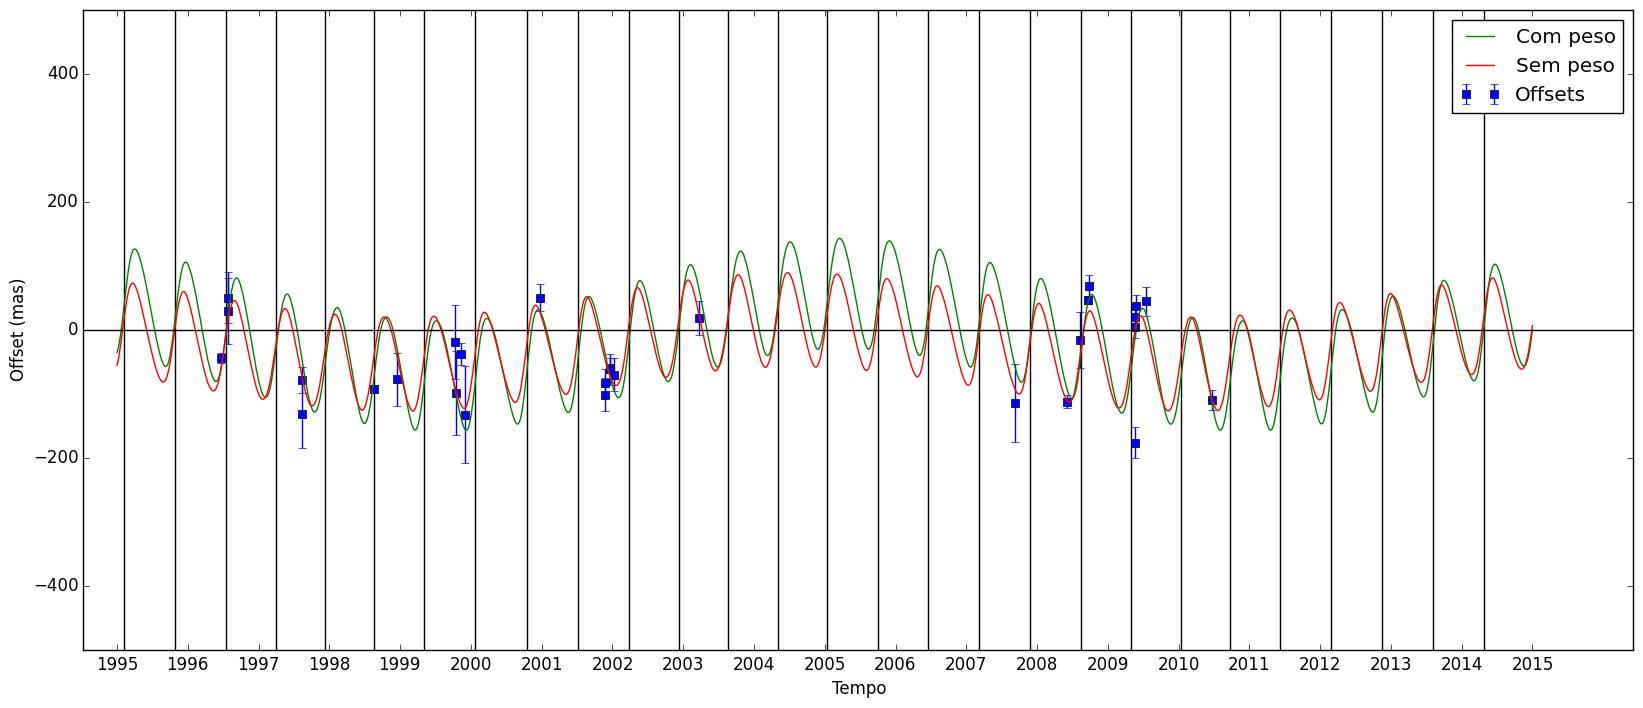
\includegraphics[scale=0.35]{Lysithea/DEC.png} 
\end{figure}

\begin{figure}[h]
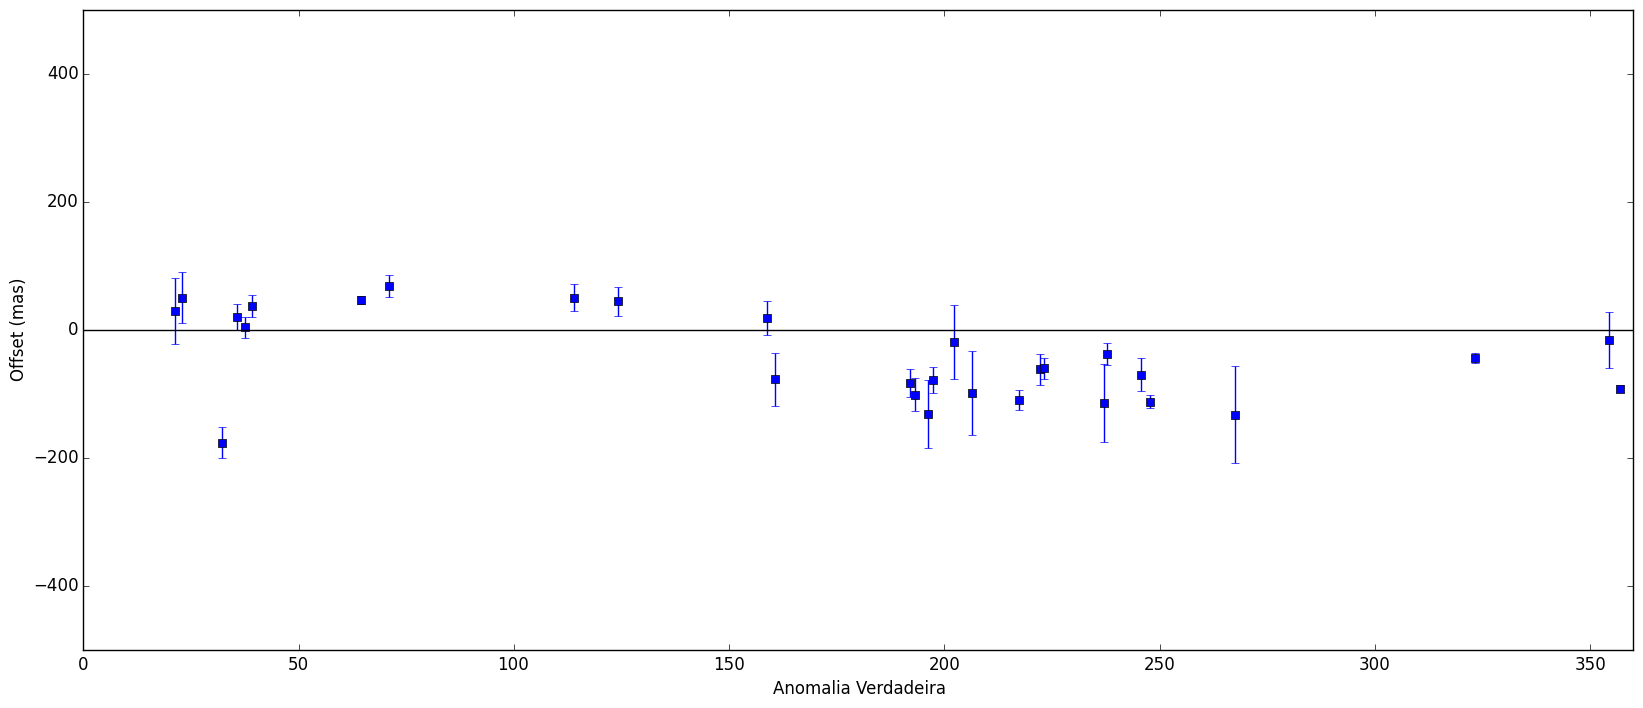
\includegraphics[scale=0.35]{Lysithea/DEC_anom.png}  
\end{figure}

\begin{table}[h!]
\caption{\label{Tab: Lysithea-DEC} Resultados dos ajustes para Lysithea - DEC}
\begin{centering}
\begin{tabular}{cccc}
\hline
\hline
Parâmetro & Com peso & Sem peso & Unidade\tabularnewline
\hline
p[0] & 64 $\pm$ 20 & 34 $\pm$ 24 & mas\\
p[1] & 11.3 $\pm$ 0.7 & 11.1 $\pm$ 1.9 & anos\\
p[2] & -1.3 $\pm$ 0.3 & -1.0 $\pm$ 0.5 & rad\\
p[3] & 85 $\pm$ 14 & 72 $\pm$ 17 & mas\\
p[4] & -12 $\pm$ 15 & 11 $\pm$ 16 & mas\\
p[5] & -8 $\pm$ 14 & -19 $\pm$ 15 & mas\\
Residuo & 267 & 249 & mas\\
\hline 
\end{tabular} 
\par\end{centering}
\end{table}

\chapter*{Sinope}
\section*{Ascensão Reta}

\begin{figure}[h]
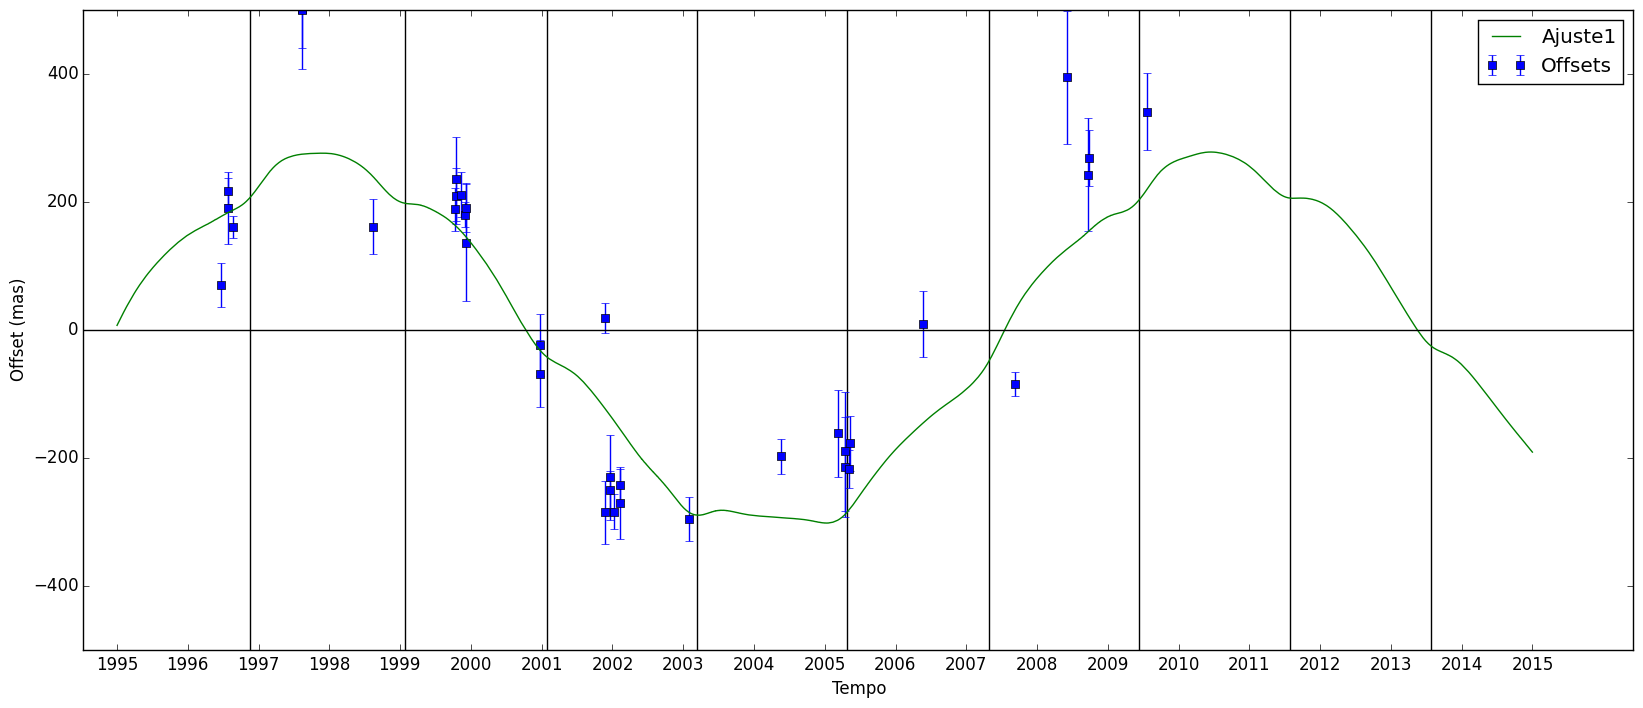
\includegraphics[scale=0.35]{Sinope/RA.png} 
\end{figure}

\begin{figure}[h]
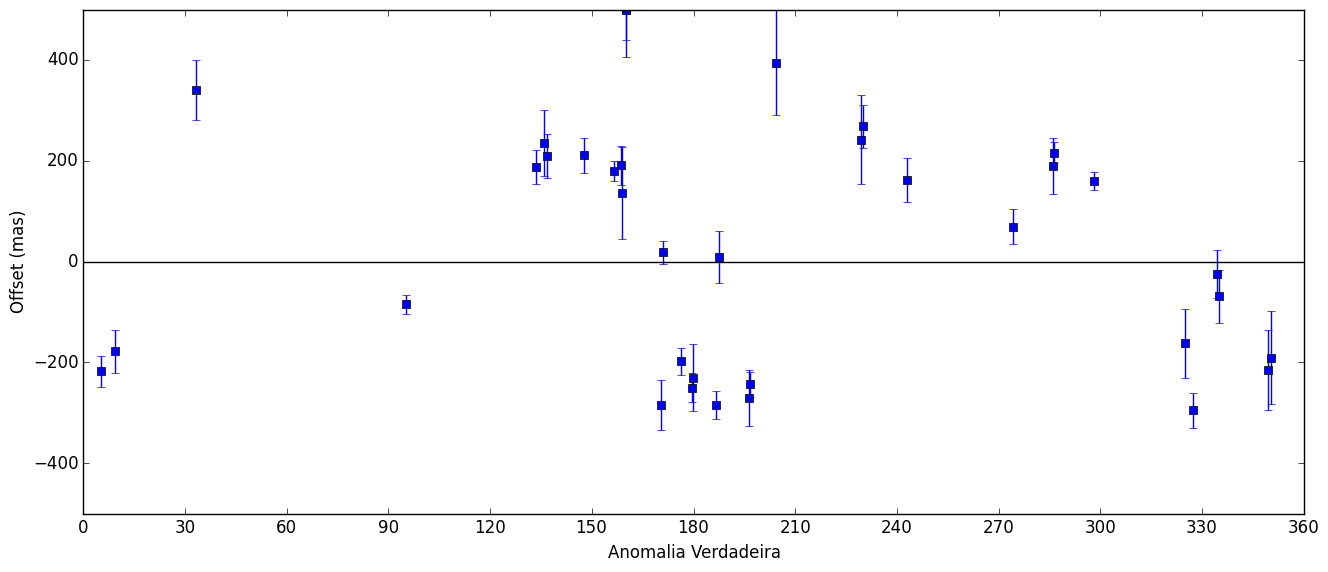
\includegraphics[scale=0.35]{Sinope/RA_anom.png}  
\end{figure}

\begin{table}[h!]
\caption{\label{Tab: Sinope-RA} Resultados dos ajustes para Sinope - RA}
\begin{centering}
\begin{tabular}{cccc}
\hline
\hline
Parâmetro & Com peso & Sem peso & Unidade\tabularnewline
\hline
p[0] & -284 $\pm$ 28 & -316 $\pm$ 25 & mas\\
p[1] & 12 $\pm$ 1 & 11.7 $\pm$ 0.7 & anos\\
p[2] & -0.5 $\pm$ 0.1 & -0.4 $\pm$ 0.1 & rad\\
p[3] & 10 $\pm$ 48 & 44 $\pm$ 37 & mas\\
p[4] & -15 $\pm$ 31 & -18 $\pm$ 24 & mas\\
p[5] & -26 $\pm$ 21 & 1 $\pm$ 21 & mas\\
Residuo & 671 & 532 & mas\\
\hline 
\end{tabular} 
\par\end{centering}
\end{table}

\section*{Declinação}

\begin{figure}[h]
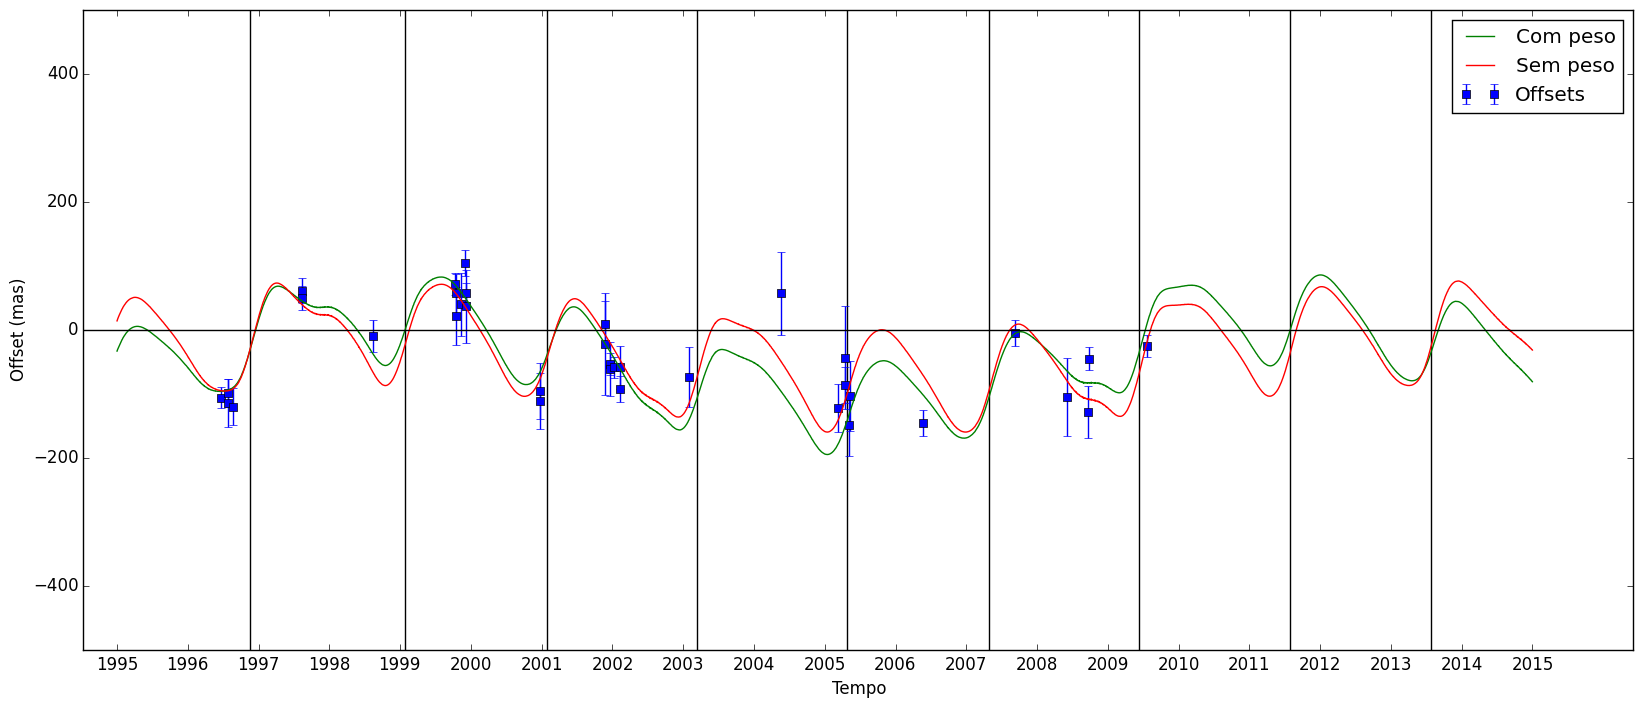
\includegraphics[scale=0.35]{Sinope/DEC.png} 
\end{figure}

\begin{figure}[h]
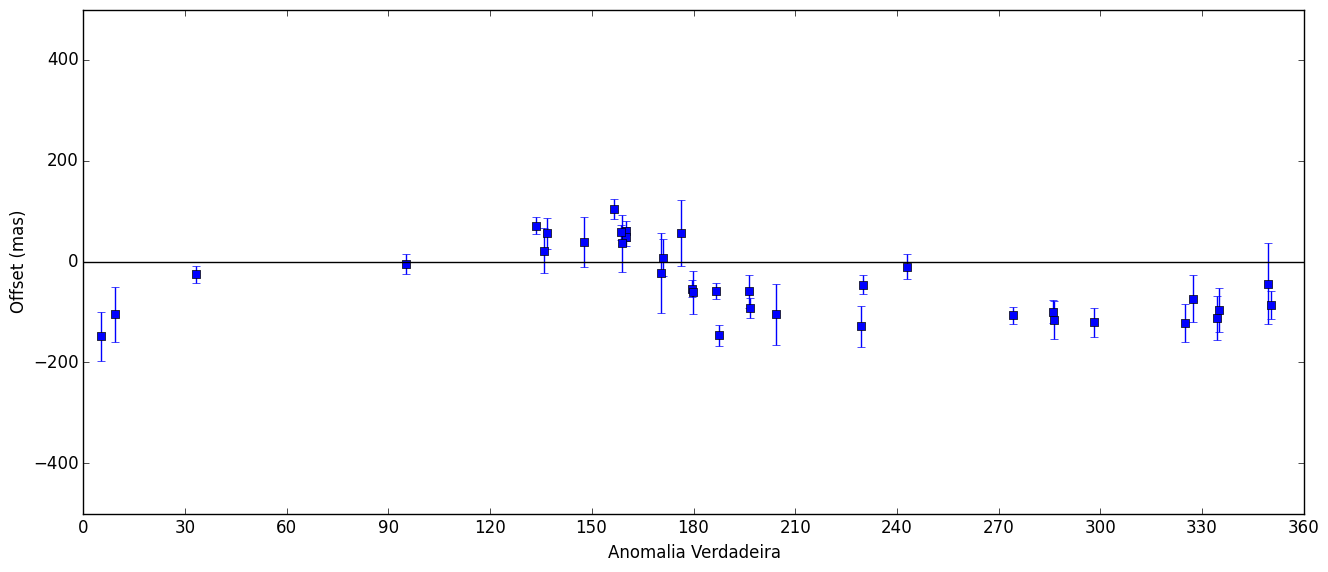
\includegraphics[scale=0.35]{Sinope/DEC_anom.png}  
\end{figure}

\begin{table}[h!]
\caption{\label{Tab: Sinope-DEC} Resultados dos ajustes para Sinope - DEC}
\begin{centering}
\begin{tabular}{cccc}
\hline
\hline
Parâmetro & Com peso & Sem peso & Unidade\tabularnewline
\hline
p[0] & -69 $\pm$ 11 & -38 $\pm$ 11 & mas\\
p[1] & 12.7 $\pm$ 0.7 & 15 $\pm$ 3 & anos\\
p[2] & 5.2 $\pm$ 0.1 & 5.4 $\pm$ 0.4 & rad\\
p[3] & 69 $\pm$ 11 & 79 $\pm$ 15 & mas\\
p[4] & -18 $\pm$ 9 & -19 $\pm$ 10 & mas\\
p[5] & -54 $\pm$ 7 & -43 $\pm$ 8 & mas\\
Residuo & 266 & 229 & mas\\
\hline 
\end{tabular} 
\par\end{centering}
\end{table}

\chapter*{Pasiphae}
\section*{Ascensão Reta}

\begin{figure}[h]
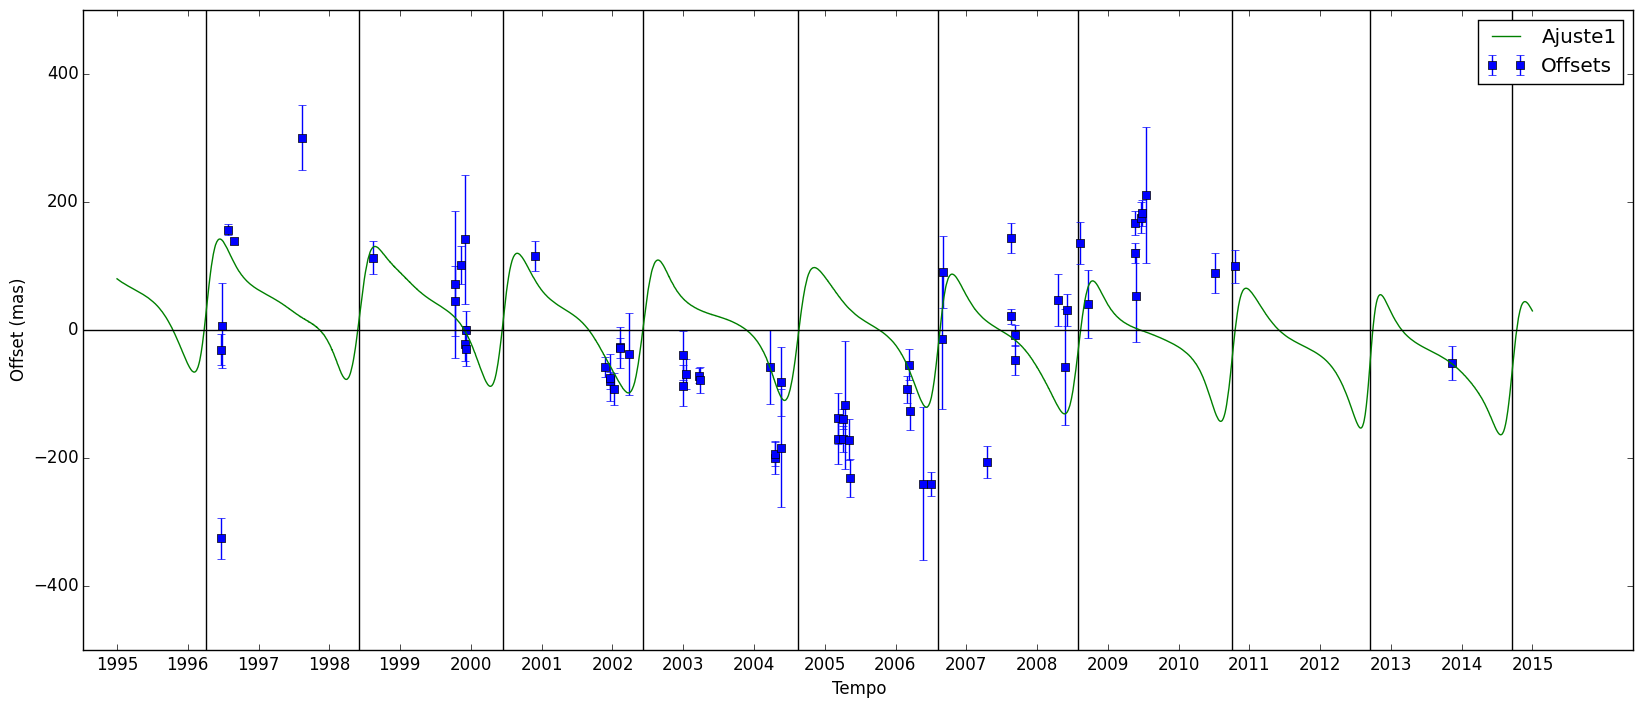
\includegraphics[scale=0.35]{Pasiphae/RA.png} 
\end{figure}

\begin{figure}[h]
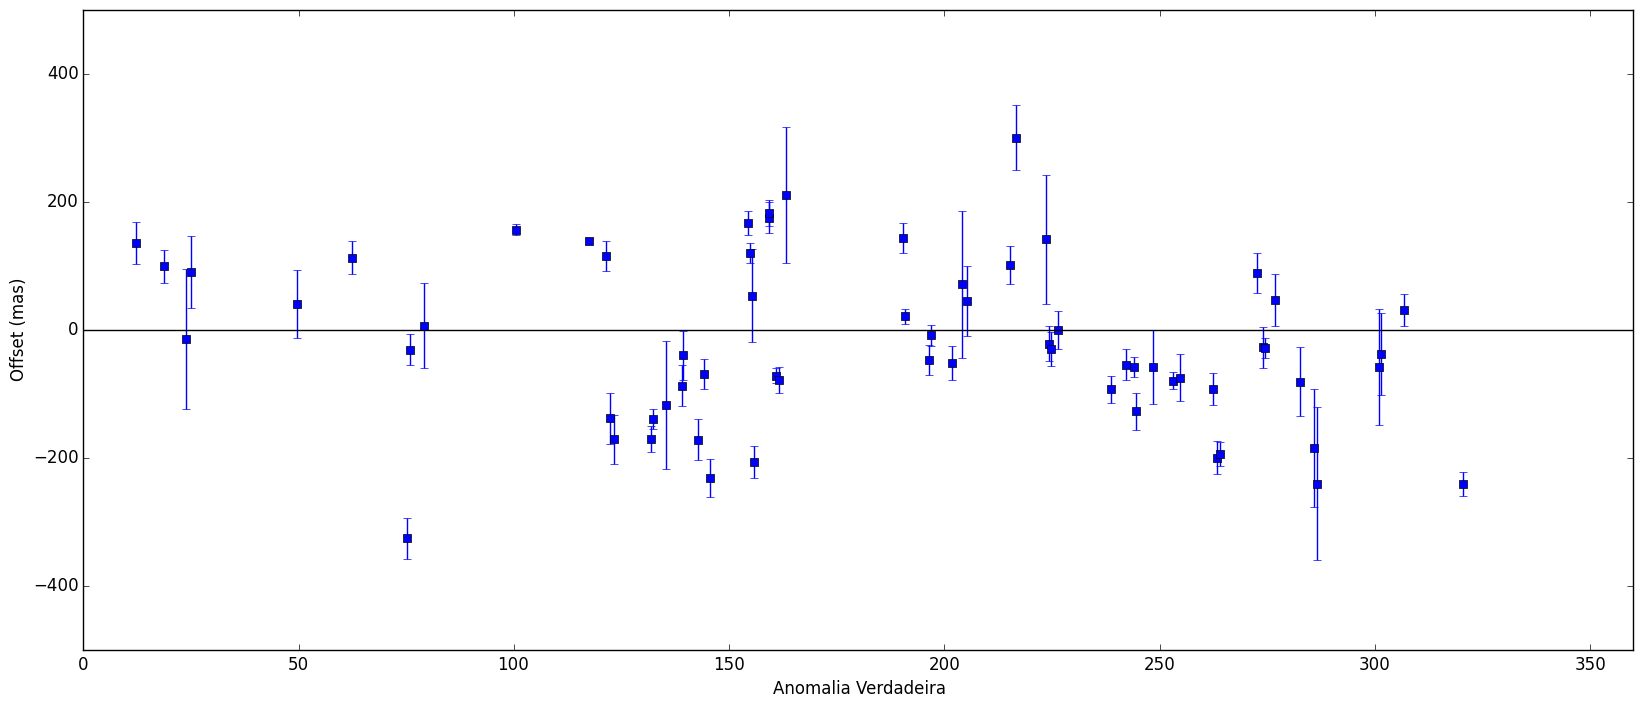
\includegraphics[scale=0.35]{Pasiphae/RA_anom.png}  
\end{figure}

\begin{table}[h!]
\caption{\label{Tab: Pasiphae-RA} Resultados dos ajustes para Pasiphae - RA}
\begin{centering}
\begin{tabular}{cccc}
\hline
\hline
Parâmetro & Com peso & Sem peso & Unidade\tabularnewline
\hline
p[0] & -157 $\pm$ 14 & -136 $\pm$ 15 & mas\\
p[1] & 12.7 $\pm$ 0.4 & 11.3 $\pm$ 0.6 & anos\\
p[2] & -0.6 $\pm$ 0.1 & -1.0 $\pm$ 0.1 & rad\\
p[3] & 20 $\pm$ 16 & 15 $\pm$ 17 & mas\\
p[4] & -39 $\pm$ 19 & -16 $\pm$ 19 & mas\\
p[5] & -17 $\pm$ 12 & -24 $\pm$ 13 & mas\\
Residuo & 733 & 679 & mas\\
\hline 
\end{tabular} 
\par\end{centering}
\end{table}

\section*{Declinação}

\begin{figure}[h]
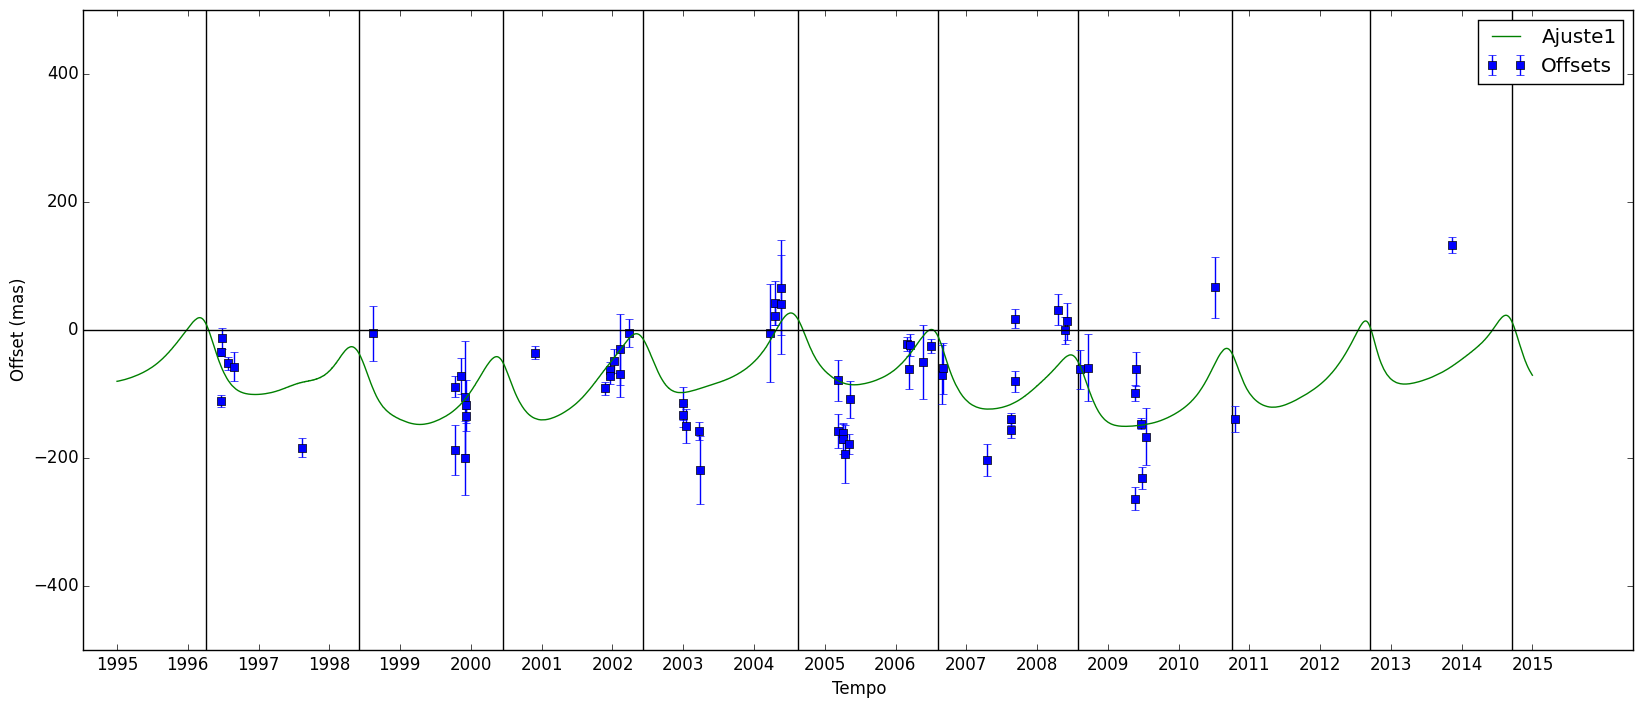
\includegraphics[scale=0.35]{Pasiphae/DEC.png} 
\end{figure}

\begin{figure}[h]
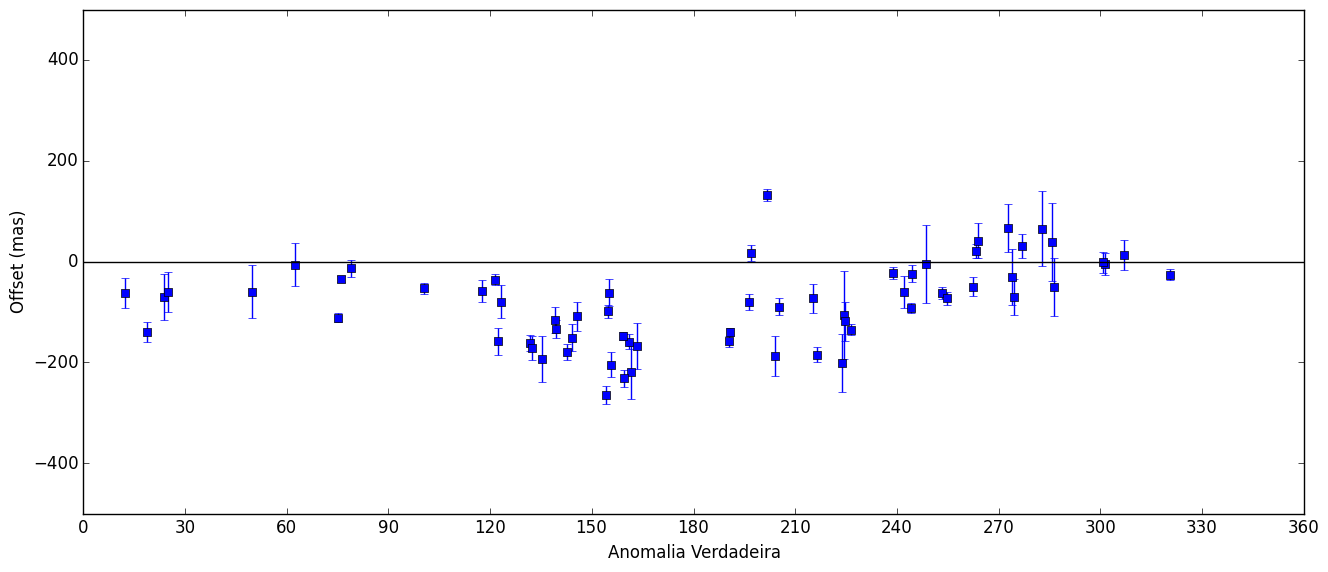
\includegraphics[scale=0.35]{Pasiphae/DEC_anom.png}  
\end{figure}

\begin{table}[h!]
\caption{\label{Tab: Pasiphae-DEC} Resultados dos ajustes para Pasiphae - DEC}
\begin{centering}
\begin{tabular}{cccc}
\hline
\hline
Parâmetro & Com peso & Sem peso & Unidade\tabularnewline
\hline
p[0] & 35 $\pm$ 13 & 26 $\pm$ 10 & mas\\
p[1] & 9 $\pm$ 1 & 8 $\pm$ 2 & anos\\
p[2] & -1.5 $\pm$ 0.5 & -1.9 $\pm$ 0.8 & rad\\
p[3] & -30 $\pm$ 14 & -48 $\pm$ 11 & mas\\
p[4] & 44 $\pm$ 16 & 58 $\pm$ 13 & mas\\
p[5] & -62 $\pm$ 10 & -67 $\pm$ 9 & mas\\
Residuo & 513 & 488 & mas\\
\hline 
\end{tabular} 
\par\end{centering}
\end{table}

\chapter*{Phoebe}
\section*{Ascensão Reta}

\begin{figure}[h]
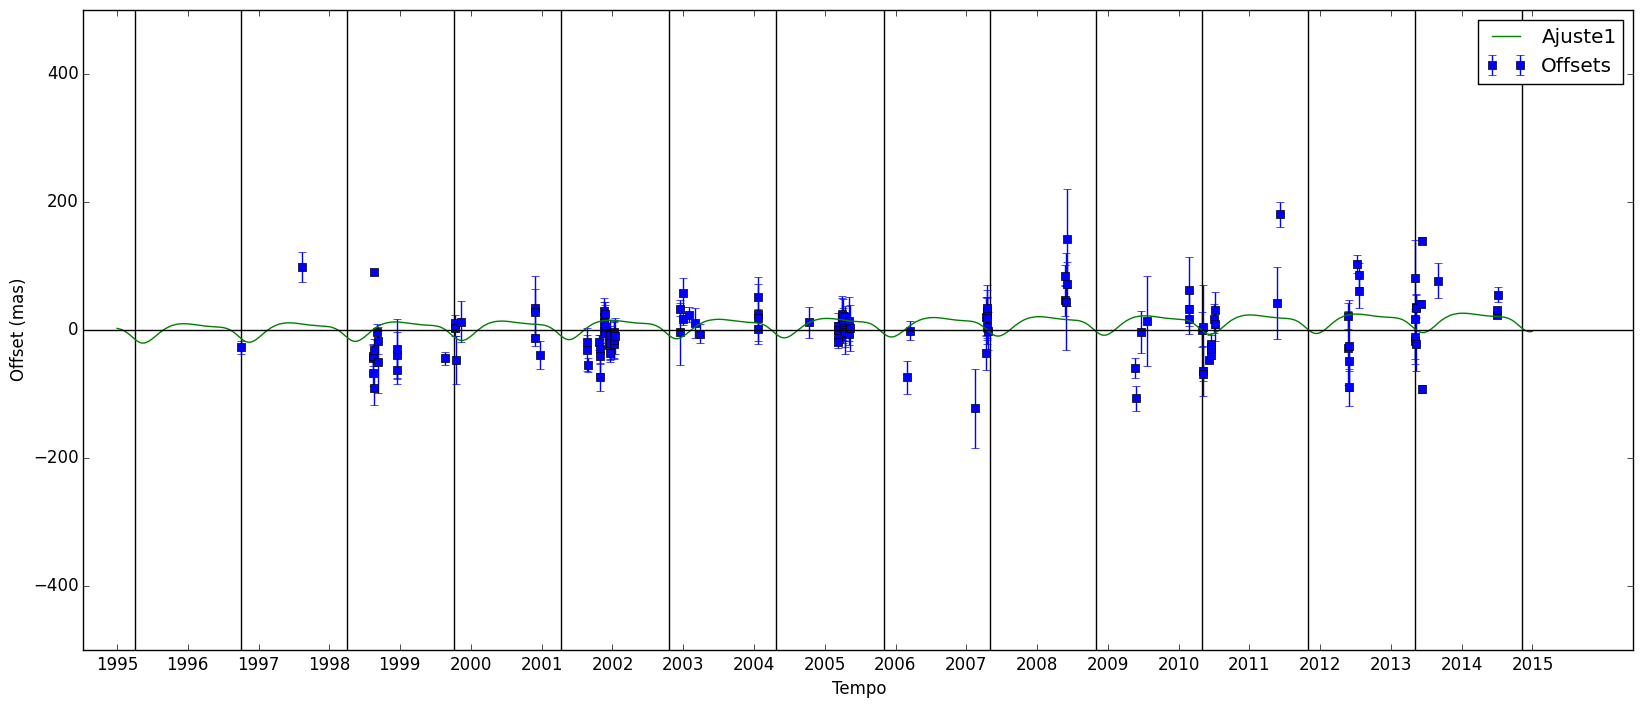
\includegraphics[scale=0.35]{Phoebe/RA.png} 
\end{figure}

\begin{figure}[h]
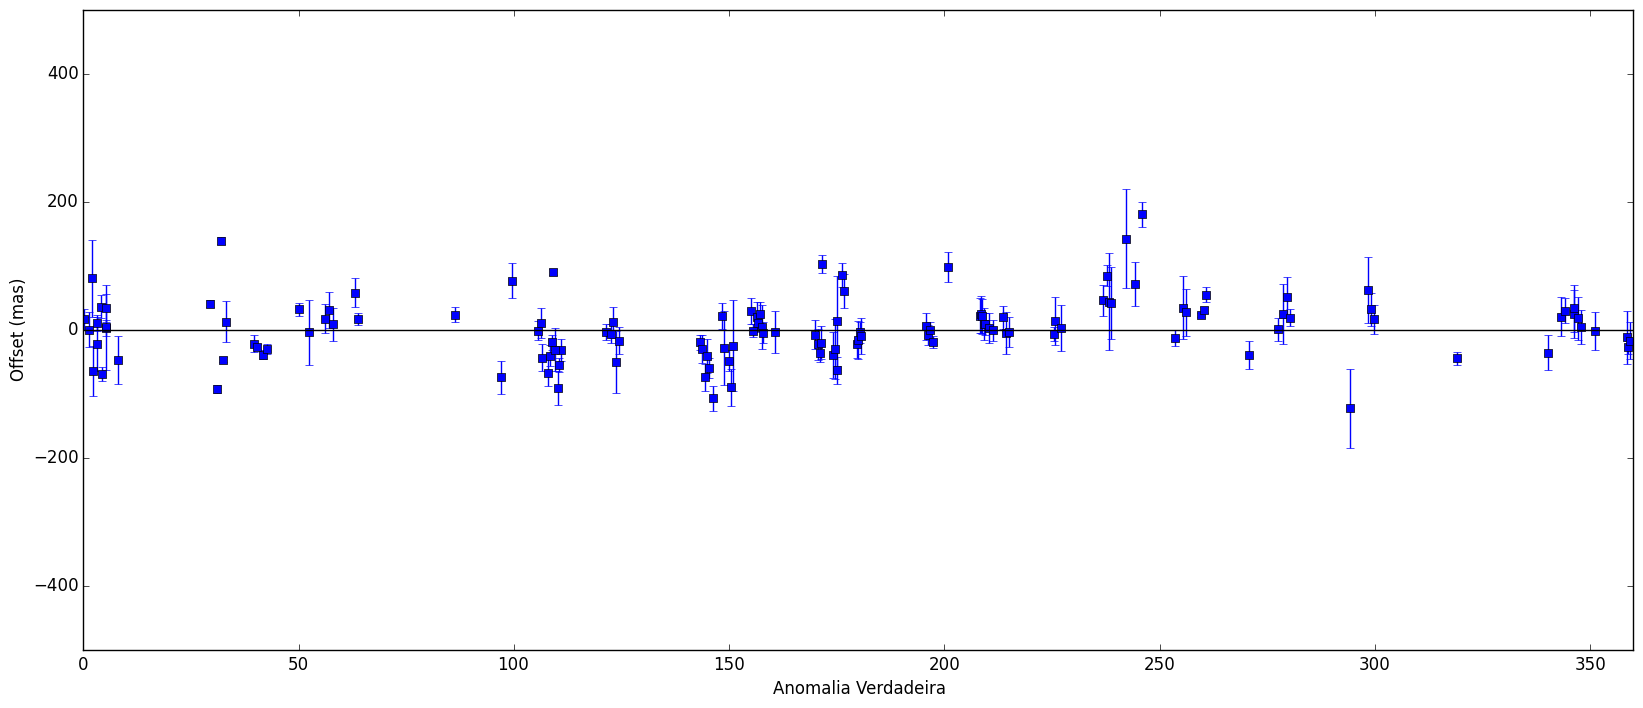
\includegraphics[scale=0.35]{Phoebe/RA_anom.png}  
\end{figure}

\begin{table}[h!]
\caption{\label{Tab: Phoebe-RA} Resultados dos ajustes para Phoebe - RA}
\begin{centering}
\begin{tabular}{cccc}
\hline
\hline
Parâmetro & Com peso & Sem peso & Unidade\tabularnewline
\hline
p[0] & -17 $\pm$ 8 & -17 $\pm$ 8 & mas\\
p[1] & 0.99 $\pm$ 0.01 & 1.01 $\pm$ 0.01 & anos\\
p[2] & 0.6 $\pm$ 0.8 & 1.9 $\pm$ 0.5 & rad\\
p[3] & -8. $\pm$ 7 & -26 $\pm$ 6 & mas\\
p[4] & -12 $\pm$ 8 & 1 $\pm$ 5 & mas\\
p[5] & 2 $\pm$ 9 & 8 $\pm$ 8 & mas\\
Residuo & 551 & 505 & mas\\
\hline 
\end{tabular} 
\par\end{centering}
\end{table}

\section*{Declinação}

\begin{figure}[h]
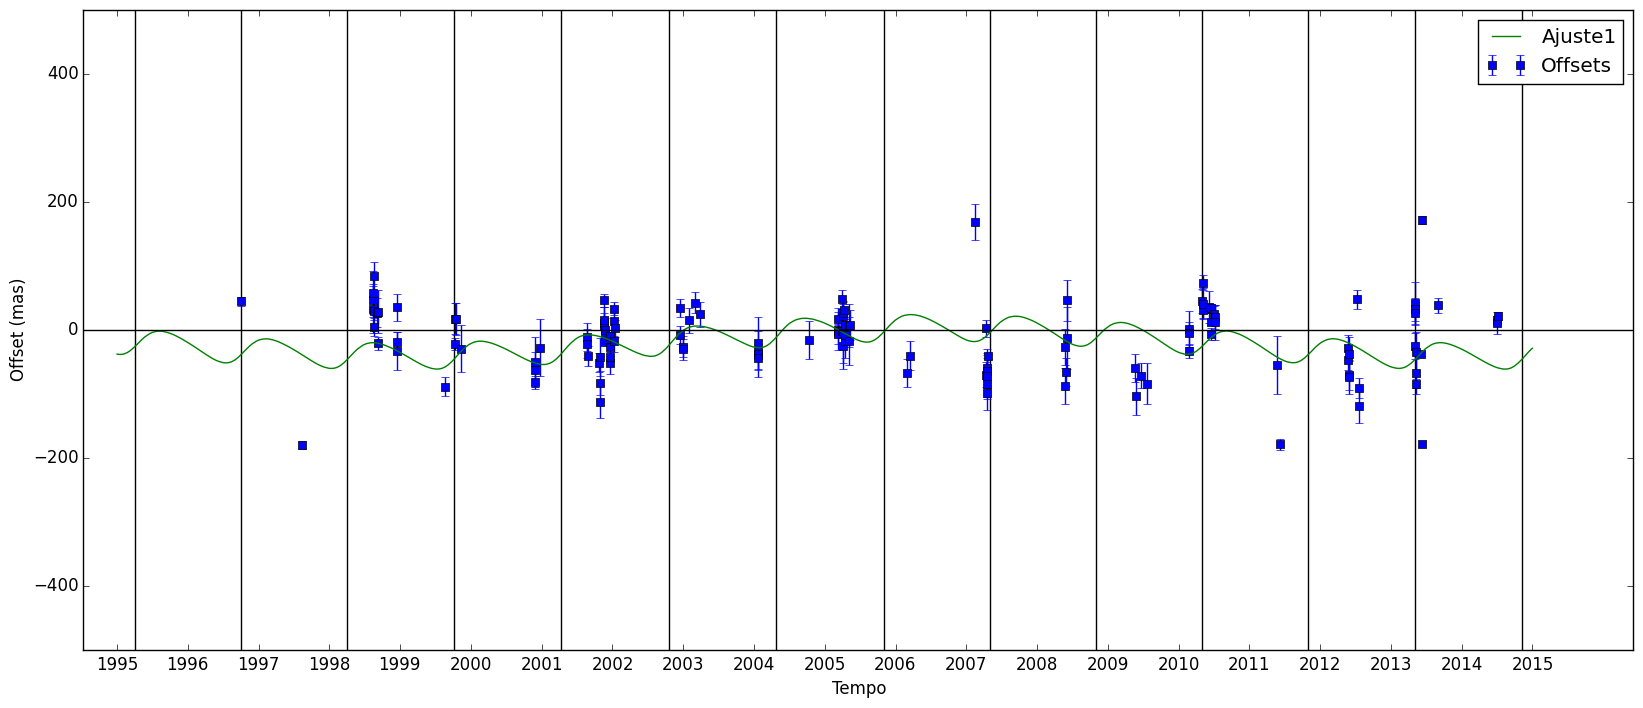
\includegraphics[scale=0.35]{Phoebe/DEC.png} 
\end{figure}

\begin{figure}[h]
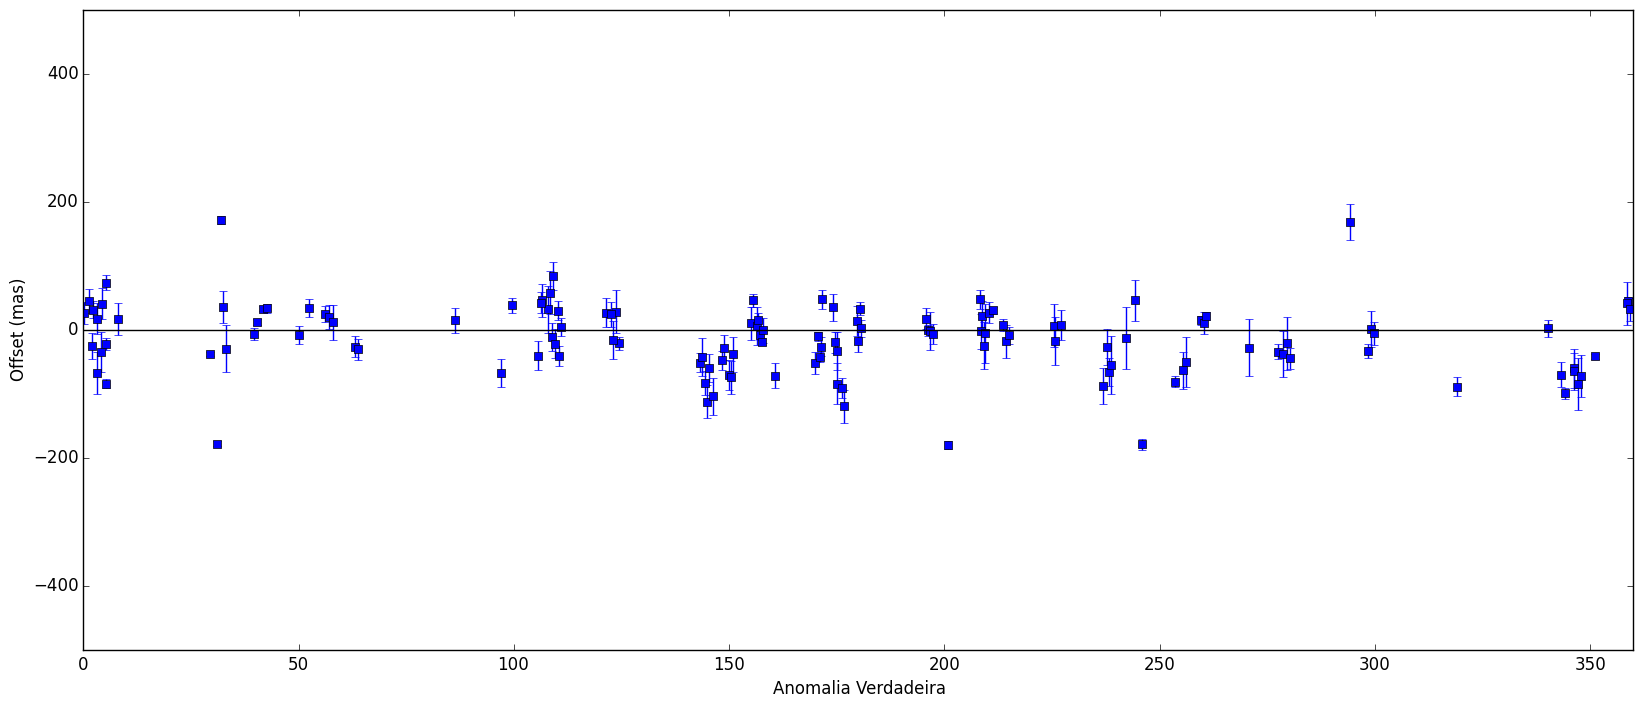
\includegraphics[scale=0.35]{Phoebe/DEC_anom.png}  
\end{figure}

\begin{table}[h!]
\caption{\label{Tab: Phoebe-DEC} Resultados dos ajustes para Phoebe - DEC}
\begin{centering}
\begin{tabular}{cccc}
\hline
\hline
Parâmetro & Com peso & Sem peso & Unidade\tabularnewline
\hline
p[0] & 22 $\pm$ 14 & 20 $\pm$ 8 & mas\\
p[1] & 0.97 $\pm$ 0.01 & 0.95 $\pm$ 0.01 & anos\\
p[2] & 0.4 $\pm$ 0.7 & -0.6 $\pm$ 0.4 & rad\\
p[3] & 17 $\pm$ 12 & 16 $\pm$ 7 & mas\\
p[4] & 2 $\pm$ 10 & 10 $\pm$ 6 & mas\\
p[5] & -16 $\pm$ 8 & -9 $\pm$ 5 & mas\\
Residuo & 618 & 594 & mas\\
\hline 
\end{tabular} 
\par\end{centering}
\end{table}

\chapter*{Nereida}
\section*{Ascensão Reta}

\begin{figure}[h]
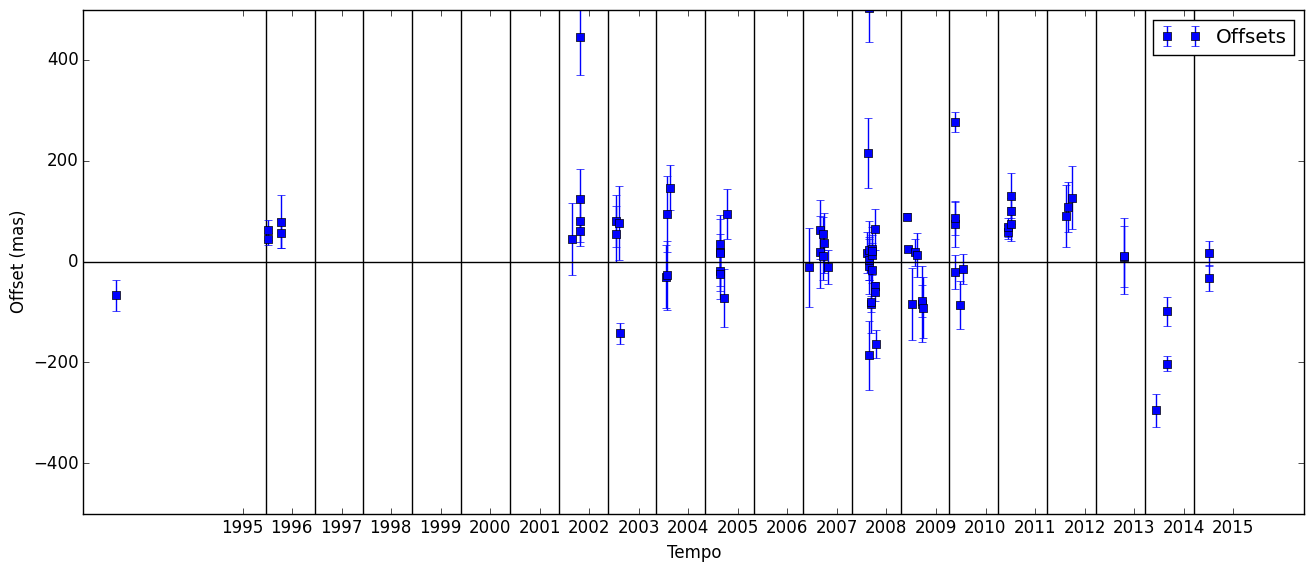
\includegraphics[scale=0.35]{Nereida/RA.png} 
\end{figure}

\begin{figure}[h]
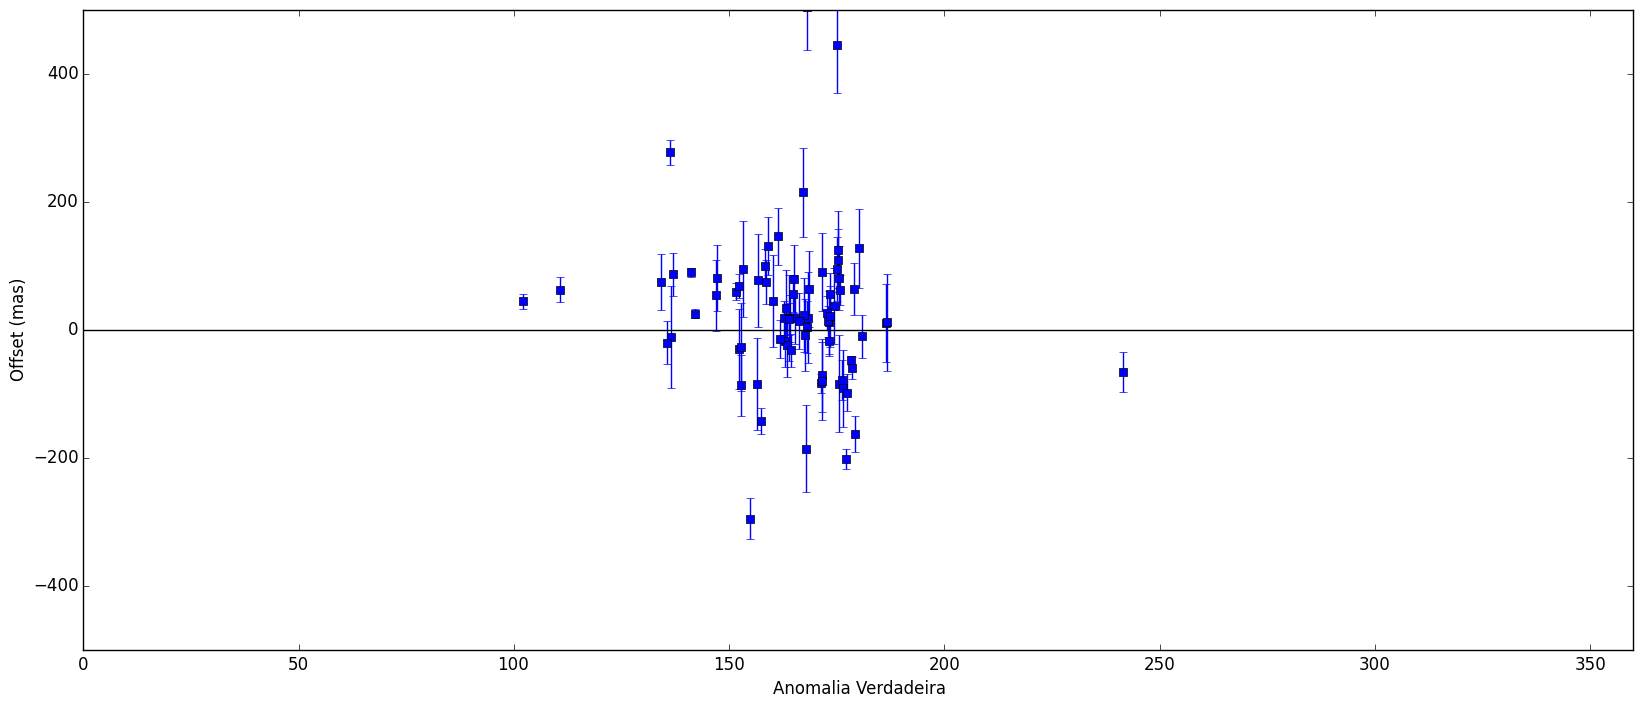
\includegraphics[scale=0.35]{Nereida/RA_anom.png}  
\end{figure}

\begin{table}[h!]
\caption{\label{Tab: Nereida-RA} Resultados dos ajustes para Nereida - RA}
\begin{centering}
\begin{tabular}{cccc}
\hline
\hline
Parâmetro & Com peso & Sem peso & Unidade\tabularnewline
\hline
p[0] & -130 $\pm$ 29 & -46 $\pm$ 25 & mas\\
p[1] & 11.3 $\pm$ 0.7 & 8 $\pm$ 1 & anos\\
p[2] & -0.8 $\pm$ 0.3 & -2.8 $\pm$ 0.9 & rad\\
p[3] & 39 $\pm$ 81 & 39 $\pm$ 81 & mas\\
p[4] & 193 $\pm$ 119 & -27 $\pm$ 130 & mas\\
p[5] & 123 $\pm$ 125 & -21 $\pm$ 130 & mas\\
Residuo & 1427 & 1154 & mas\\
\hline 
\end{tabular} 
\par\end{centering}
\end{table}

\section*{Declinação}

\begin{figure}[h]
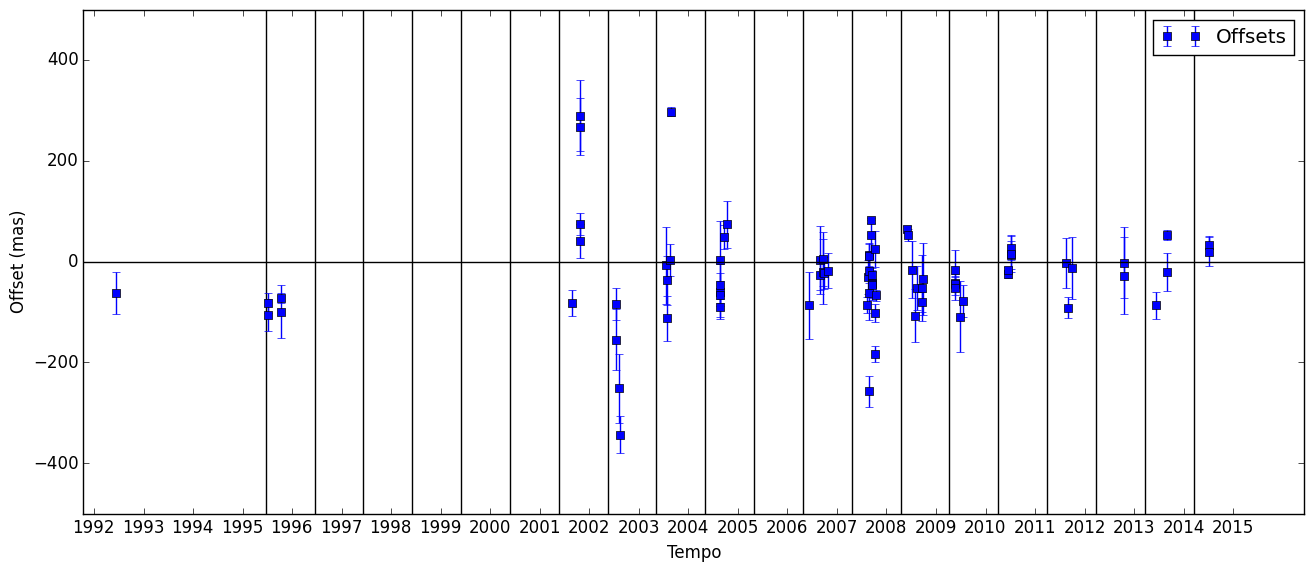
\includegraphics[scale=0.35]{Nereida/DEC.png} 
\end{figure}

\begin{figure}[h]
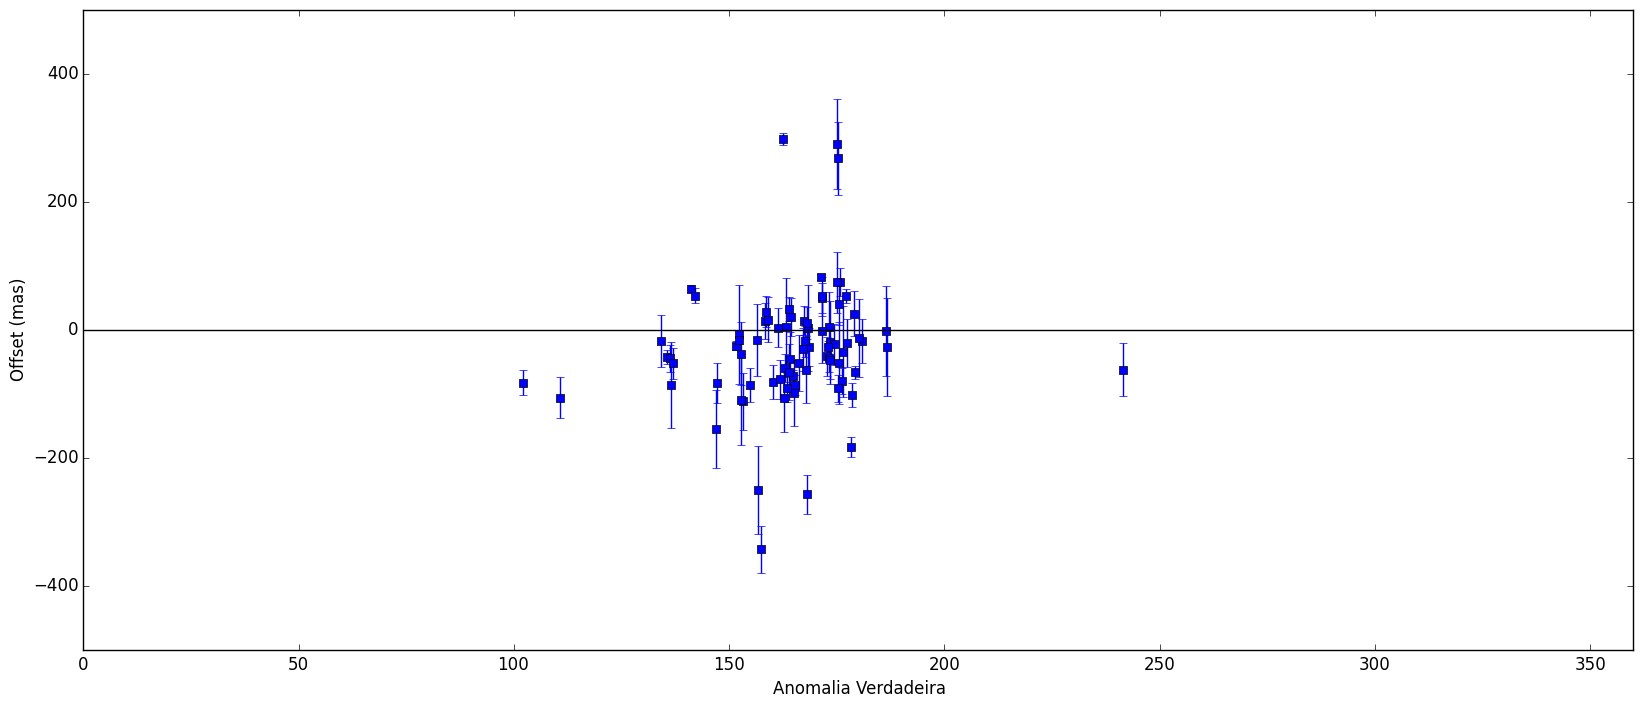
\includegraphics[scale=0.35]{Nereida/DEC_anom.png}  
\end{figure}

\begin{table}[h!]
\caption{\label{Tab: Nereida-Dec} Resultados dos ajustes para Nereida - DEC}
\begin{centering}
\begin{tabular}{cccc}
\hline
\hline
Parâmetro & Com peso & Sem peso & Unidade\tabularnewline
\hline
p[0] & 83 $\pm$ 19 & 21 $\pm$ 17 & mas\\
p[1] & 14 $\pm$ 2 & -14 $\pm$ 7 & anos\\
p[2] & -0.1 $\pm$ 0.6 & 1.9 $\pm$ 1.7 & rad\\
p[3] & 165 $\pm$ 87 & -40 $\pm$ 51 & mas\\
p[4] & -186 $\pm$ 158 & -63 $\pm$ 92 & mas\\
p[5] & -182 $\pm$ 172 & -70 $\pm$ 93 & mas\\
Residuo & 1120 & 820 & mas\\
\hline 
\end{tabular} 
\par\end{centering}
\end{table}

\end{document}